% Options for packages loaded elsewhere
% Options for packages loaded elsewhere
\PassOptionsToPackage{unicode}{hyperref}
\PassOptionsToPackage{hyphens}{url}
\PassOptionsToPackage{dvipsnames,svgnames,x11names}{xcolor}
%
\documentclass[
  12pt,
  titlepage]{article}
\usepackage{xcolor}
\usepackage[margin=2.5cm]{geometry}
\usepackage{amsmath,amssymb}
\setcounter{secnumdepth}{5}
\usepackage{iftex}
\ifPDFTeX
  \usepackage[T1]{fontenc}
  \usepackage[utf8]{inputenc}
  \usepackage{textcomp} % provide euro and other symbols
\else % if luatex or xetex
  \usepackage{unicode-math} % this also loads fontspec
  \defaultfontfeatures{Scale=MatchLowercase}
  \defaultfontfeatures[\rmfamily]{Ligatures=TeX,Scale=1}
\fi
\usepackage{lmodern}
\ifPDFTeX\else
  % xetex/luatex font selection
\fi
% Use upquote if available, for straight quotes in verbatim environments
\IfFileExists{upquote.sty}{\usepackage{upquote}}{}
\IfFileExists{microtype.sty}{% use microtype if available
  \usepackage[]{microtype}
  \UseMicrotypeSet[protrusion]{basicmath} % disable protrusion for tt fonts
}{}
\makeatletter
\@ifundefined{KOMAClassName}{% if non-KOMA class
  \IfFileExists{parskip.sty}{%
    \usepackage{parskip}
  }{% else
    \setlength{\parindent}{0pt}
    \setlength{\parskip}{6pt plus 2pt minus 1pt}}
}{% if KOMA class
  \KOMAoptions{parskip=half}}
\makeatother
% Make \paragraph and \subparagraph free-standing
\makeatletter
\ifx\paragraph\undefined\else
  \let\oldparagraph\paragraph
  \renewcommand{\paragraph}{
    \@ifstar
      \xxxParagraphStar
      \xxxParagraphNoStar
  }
  \newcommand{\xxxParagraphStar}[1]{\oldparagraph*{#1}\mbox{}}
  \newcommand{\xxxParagraphNoStar}[1]{\oldparagraph{#1}\mbox{}}
\fi
\ifx\subparagraph\undefined\else
  \let\oldsubparagraph\subparagraph
  \renewcommand{\subparagraph}{
    \@ifstar
      \xxxSubParagraphStar
      \xxxSubParagraphNoStar
  }
  \newcommand{\xxxSubParagraphStar}[1]{\oldsubparagraph*{#1}\mbox{}}
  \newcommand{\xxxSubParagraphNoStar}[1]{\oldsubparagraph{#1}\mbox{}}
\fi
\makeatother


\usepackage{longtable,booktabs,array}
\usepackage{calc} % for calculating minipage widths
% Correct order of tables after \paragraph or \subparagraph
\usepackage{etoolbox}
\makeatletter
\patchcmd\longtable{\par}{\if@noskipsec\mbox{}\fi\par}{}{}
\makeatother
% Allow footnotes in longtable head/foot
\IfFileExists{footnotehyper.sty}{\usepackage{footnotehyper}}{\usepackage{footnote}}
\makesavenoteenv{longtable}
\usepackage{graphicx}
\makeatletter
\newsavebox\pandoc@box
\newcommand*\pandocbounded[1]{% scales image to fit in text height/width
  \sbox\pandoc@box{#1}%
  \Gscale@div\@tempa{\textheight}{\dimexpr\ht\pandoc@box+\dp\pandoc@box\relax}%
  \Gscale@div\@tempb{\linewidth}{\wd\pandoc@box}%
  \ifdim\@tempb\p@<\@tempa\p@\let\@tempa\@tempb\fi% select the smaller of both
  \ifdim\@tempa\p@<\p@\scalebox{\@tempa}{\usebox\pandoc@box}%
  \else\usebox{\pandoc@box}%
  \fi%
}
% Set default figure placement to htbp
\def\fps@figure{htbp}
\makeatother


% definitions for citeproc citations
\NewDocumentCommand\citeproctext{}{}
\NewDocumentCommand\citeproc{mm}{%
  \begingroup\def\citeproctext{#2}\cite{#1}\endgroup}
\makeatletter
 % allow citations to break across lines
 \let\@cite@ofmt\@firstofone
 % avoid brackets around text for \cite:
 \def\@biblabel#1{}
 \def\@cite#1#2{{#1\if@tempswa , #2\fi}}
\makeatother
\newlength{\cslhangindent}
\setlength{\cslhangindent}{1.5em}
\newlength{\csllabelwidth}
\setlength{\csllabelwidth}{3em}
\newenvironment{CSLReferences}[2] % #1 hanging-indent, #2 entry-spacing
 {\begin{list}{}{%
  \setlength{\itemindent}{0pt}
  \setlength{\leftmargin}{0pt}
  \setlength{\parsep}{0pt}
  % turn on hanging indent if param 1 is 1
  \ifodd #1
   \setlength{\leftmargin}{\cslhangindent}
   \setlength{\itemindent}{-1\cslhangindent}
  \fi
  % set entry spacing
  \setlength{\itemsep}{#2\baselineskip}}}
 {\end{list}}
\usepackage{calc}
\newcommand{\CSLBlock}[1]{\hfill\break\parbox[t]{\linewidth}{\strut\ignorespaces#1\strut}}
\newcommand{\CSLLeftMargin}[1]{\parbox[t]{\csllabelwidth}{\strut#1\strut}}
\newcommand{\CSLRightInline}[1]{\parbox[t]{\linewidth - \csllabelwidth}{\strut#1\strut}}
\newcommand{\CSLIndent}[1]{\hspace{\cslhangindent}#1}



\setlength{\emergencystretch}{3em} % prevent overfull lines

\providecommand{\tightlist}{%
  \setlength{\itemsep}{0pt}\setlength{\parskip}{0pt}}



 


\usepackage{booktabs}
\usepackage{longtable}
\usepackage{array}
\usepackage{multirow}
\usepackage{wrapfig}
\usepackage{float}
\usepackage{colortbl}
\usepackage{pdflscape}
\usepackage{tabu}
\usepackage{threeparttable}
\usepackage{threeparttablex}
\usepackage[normalem]{ulem}
\usepackage{makecell}
\usepackage{xcolor}
\usepackage{authblk}
\renewcommand\Affilfont{\small\itshape}
\renewcommand\Authfont{\normalsize}
\author[1]{Adam Dennett\thanks{a.dennett@ucl.ac.uk, ORCID: 0000-0002-7493-3276}}
\author[3]{Dan Campbell-Meiklejohn\thanks{daniel.cm@sussex.ac.uk, ORCID: 0000-0002-8916-265X}}
\author[1]{Beatrice Taylor\thanks{beatrice.taylor@ucl.ac.uk, ORCID: 0000-0002-3630-5047 }}
\affil[1]{Bartlett Centre for Advanced Spatial Analysis, University College London}
\affil[3]{School of Psychology, University of Sussex}
\renewcommand{\author}[2][]{}
\renewcommand{\and}{}
\makeatletter
\@ifpackageloaded{caption}{}{\usepackage{caption}}
\AtBeginDocument{%
\ifdefined\contentsname
  \renewcommand*\contentsname{Table of contents}
\else
  \newcommand\contentsname{Table of contents}
\fi
\ifdefined\listfigurename
  \renewcommand*\listfigurename{List of Figures}
\else
  \newcommand\listfigurename{List of Figures}
\fi
\ifdefined\listtablename
  \renewcommand*\listtablename{List of Tables}
\else
  \newcommand\listtablename{List of Tables}
\fi
\ifdefined\figurename
  \renewcommand*\figurename{Figure}
\else
  \newcommand\figurename{Figure}
\fi
\ifdefined\tablename
  \renewcommand*\tablename{Table}
\else
  \newcommand\tablename{Table}
\fi
}
\@ifpackageloaded{float}{}{\usepackage{float}}
\floatstyle{ruled}
\@ifundefined{c@chapter}{\newfloat{codelisting}{h}{lop}}{\newfloat{codelisting}{h}{lop}[chapter]}
\floatname{codelisting}{Listing}
\newcommand*\listoflistings{\listof{codelisting}{List of Listings}}
\makeatother
\makeatletter
\makeatother
\makeatletter
\@ifpackageloaded{caption}{}{\usepackage{caption}}
\@ifpackageloaded{subcaption}{}{\usepackage{subcaption}}
\makeatother
\usepackage{bookmark}
\IfFileExists{xurl.sty}{\usepackage{xurl}}{} % add URL line breaks if available
\urlstyle{same}
\hypersetup{
  pdftitle={How to Pull the Right Lever: School Attainment, Open Data Analytics and Local Education Policy in England},
  pdfauthor={Adam Dennett; Dan Campbell-Meiklejohn; Beatrice Taylor},
  pdfkeywords={school attainment, education policy, school
absence, disadvantage gap, multilevel modelling, open data},
  colorlinks=true,
  linkcolor={blue},
  filecolor={Maroon},
  citecolor={Blue},
  urlcolor={Blue},
  pdfcreator={LaTeX via pandoc}}


\title{How to Pull the Right Lever: School Attainment, Open Data
Analytics and Local Education Policy in England}
\usepackage{etoolbox}
\makeatletter
\providecommand{\subtitle}[1]{% add subtitle to \maketitle
  \apptocmd{\@title}{\par {\large #1 \par}}{}{}
}
\makeatother
\subtitle{Lessons from Brighton and Hove}
\author{Adam Dennett \and Dan Campbell-Meiklejohn \and Beatrice Taylor}
\date{2026-04-30}
\begin{document}
\maketitle
\begin{abstract}
In its 2026 White Paper, the UK government has set a worthwhile and
ambitious target to halve the disadvantage attainment gap in education.
Achieving improvements in disadvantaged student attainment requires
local education authorities to understand their local situations and the
specific drivers in their areas. But it is all too easy to pull the
wrong policy lever when the research is complex and local intelligence
is incomplete. Recent experiences in Brighton and Hove have highlighted
the gap between open data and actionable information for Policy Makers,
Schools and anyone wanting to actively contribute to statutory public
consultations. Using multilevel linear mixed effects models fitted to
all state-funded secondary schools in England over four years (2021--22
to 2024--25), we show that school-level Attainment 8 is highly
predictable from a small number of readily available variables, but
non-linearities mean understanding local context is key. We apply these
models to a case study of Brighton and Hove, where admissions policy
proposals in 2024 were designed around the premise that attainment is
reduced by lower socio-economic mixing across schools. Our analysis
suggests these proposals are unlikely to deliver the targeted gains in
disadvantaged attainment, and that the wider literature on long school
commutes points to social and educational costs that the proposals did
not consider. By contrast, Brighton and Hove has the second worst
absence rate in England, and our modelling indicates that improving
attendance in the city would be the most impactful single lever
available for raising attainment --- particularly for disadvantaged
pupils. We also introduce a school-level value-added view that allows
parents and policy makers to assess how a school is performing
\emph{over and above} the structural intake characteristics it inherits,
helping support better-informed local decisions. We introduce a new
policy simulator tool to help bridge the gap between the Department for
Education's open data and accessible, contextualised intelligence.
\end{abstract}


\section{Introduction}\label{introduction}

Pupil outcomes, including attainment, are a recurrent policy theme given
the established links to individual life outcomes (Farquharson et al.
2024) and our collective national success through measures such as
economic productivity (Grant 2017). The UK Government's 2026 schools
white paper (DfE 2026) sets ambitious targets including halving the
disadvantage attainment gap, improving attendance, reforming admissions
and tackling place-based disadvantage. These ambitions will require
local education authorities (LEAs) to understand the specific drivers of
attainment in their areas and choose interventions accordingly.

This paper argues that the Department for Education's (DfE) open data
provides most of the raw materials needed for such nuanced localised
understanding, but a crucial gap exists between data availability and
accessible, contextualised intelligence for decision makers. We
demonstrate this through an analysis of school-level attainment across
England, combined with a case study of Brighton and Hove where a policy
direction would be predicted by our model, to potentially do more harm
than good.

Brighton and Hove provides a particularly instructive case. The city
already has a distinctive and progressive admissions landscape featuring
catchment areas with a lottery tie-break for oversubscribed schools,
introduced following a secondary school closure in 2005 (Allen et al.
2013) and an admissions priority for those on Free School Meals in all
of its community schools. In 2024, the council launched proposals to
shake things up even further by reducing Published Admission Numbers at
popular central-catchment schools (and keeping them higher at less
popular under-subscribed schools), reserving a number of places for
out-of-catchment children in central catchments, ahead of in-catchment
children and altering the catchment areas in the city. These new policy
proposals were promoted to the public as premised on the assumption that
attainment in the city was `driven by economic advantage' and that
redistributing pupils around the city would narrow the attainment gap.
The response to the consultation was overwhelmingly negative from
parents and schools alike, yet many did not have the tools to
effectively challenge the proposal and the core policy direction
persisted - albeit eventually slightly watered down from the initial
proposals.

Raw data on the attainment gap, without context, was presented to the
city along with statements about the correlation between concentrations
of disadvantage in schools and lower attainment. The attainment gap was
painted by the policy makers as a unique failure in need of urgent
action to counter the assumed impact of economic advantage on school
attainment. Such was the dominance of the narrative around economic
advantage, the second-order impacts of the policy interventions, for
example longer school journeys to schools outside of local communities
affecting safety, attainment, environment and the well-being of affected
children, were not scrutinised in depth. It is our proposal that
detailed data and analytics about the local situation would have led to
a different framing of the city's situation. Some rapidly produced
analysis was put into the public domain by some of the authors of this
paper\footnote{\url{https://adamdennett.github.io/BH_Schools_Consultation/about.html}},
but this was produced as a response to, rather than contributing to, the
creation of the policy. Consistent with the national picture, there is
an attainment gap in Brighton and Hove. However, what we (the citizens
of Brighton and Hove, including the local councillors developing policy)
didn't know at the time, was prior to the policy proposals, Brighton and
Hove was one of the best performing Local Education Authorities in the
Country for both disadvantaged (7th out of 152) and non-disadvantaged
(5th out of 152) GCSE attainment, once you account for the factors we
know influence that attainment. With this knowledge, the approach to
improving outcomes for disadvantaged pupils could have been more
effective by asking, for example, ``what can we learn from what the city
is doing right?'' and ``would asking pupils to travel out of their
communities to schools jeopardise this success?'' While we can't know if
open, accessible, location-specific analysis would have resulted in a
change of policy direction, it would have facilitated far more informed
policy debate.

The discussions that led to this paper took place over an 18 month
period spanning the 2024 and 2025 secondary school admissions
consultation in the city with a wide group of parents and stakeholders.
Some were academics, some experienced in national policy making, some
involved in school governance and teaching, others worked for the
council in different capacities and others would simply identify as
concerned parents. This diverse positionality motivates the analysis: we
argue that better analytical tools, applied to readily available open
data, could have substantially improved the quality of the policy debate
and may have resulted in better policy formation.

We are not claiming that the model outlined in this paper is the best
possible or that our variable selection is optimal, or indeed novel (the
variables and effects are very similar to those reported by Macleod et
al. (2015) over 10 years ago). Our intention is to show that with open,
freely available data and variables that are along the right lines, it
is possible to build a model explaining over 80\% of the variation in
school-level attainment with just a handful of predictors. Then, when we
know the vast majority of influences on attainment and how they interact
in different local contexts, we can answer locally targeted questions
such as: `is changing the social mix in schools likely to improve
disadvantaged pupil attainment?', `what is the most important factor
affecting attainment in a particular LEA?', and `which schools are doing
better or worse than expected?'.

We are also acutely aware that statistical analysis does not always
translate effectively into accessible policy relevant intelligence.
While the reporting of standard deviation improvements is more
statistically sound, trying to translate such an effect into a tangible
outcome would be a challenge for most. Therefore in this paper we try to
present the effects we observe in more readily understandable GCSE
points so that they have more real-world meaning and potentially more
resonance with policy makers.

The paper proceeds as follows. We briefly review the literature on
secondary school attainment drivers, then outline our modelling approach
using DfE open data. We present results showing which factors matter
most and how they interact, before applying these findings to Brighton
and Hove. We conclude with implications for local and national education
policy.

\section{Literature review: factors affecting pupil
attainment}\label{literature-review-factors-affecting-pupil-attainment}

\subsection{Socio-economic background and
disadvantage}\label{socio-economic-background-and-disadvantage}

The Education Policy Institute's annual reports document that by the
time pupils sit their GCSEs (the General Certificate of Secondary
Education - the exam most students in England sit at age 16),
disadvantaged pupils are on average around 18 months of learning behind
their more affluent peers, a gap that narrowed modestly after 2011 but
partially reversed following the COVID-19 pandemic (Tuckett et al.
2023). It is this `attainment-gap' which has remained stubbornly
persistent for many years and that the recent government white paper has
resolved to try and tackle. The size of the gap and the reasons behind
it are complex and vary from place to place, but its existence has
spawned large volumes of literature delving into disadvantage and
attainment.

Free School Meal (FSM) eligibility serves as the standard proxy for
disadvantage, though its limitations are well established. For example,
Stopforth and Gayle (2025) demonstrate that finer-grained measures of
parental social class reveal persistent attainment gaps that FSM-based
analyses tend to understate, with the thresholds for FSM eligibility low
enough that many students who might otherwise be classed as
disadvantaged, are not included in these statistics. Despite this,
because eligibility for Free School Meals is regularly recorded at pupil
and school levels, it is frequently used as a proxy.

A crucial dimension is that inequalities in outcomes between
disadvantaged and non-disadvantaged students at GCSE level are
substantially mediated by prior attainment at National Curriculum Key
Stage 2 (KS2 - the latter stages of Primary School from ages 7 to
11\footnote{Details of English National Curriculum Key Stages
  \url{https://www.gov.uk/national-curriculum}}). Prior attainment at
KS2 reflects accumulated inequalities from before secondary school
(Stopforth and Gayle 2025), and Gorard and Siddiqui (2019) show that the
duration of disadvantage is a stronger predictor than disadvantage at
any single point. We will return to this later in the paper, however
Gorard and Siddiqui (2019) take their focus on disadvantage further and
also propose that pupils do worse in schools with higher concentrations
of disadvantage, estimating improvements in grades of 0.05--0.15
standard deviations from greater social mixing. While they don't
translate this effect, it works out at approximately one GCSE grade in
one subject (most students take around 8-10 GCSE subjects in total). One
seductive policy point they make in their paper is that additional
mixing can be achieved at `almost no cost'. However this is a conjecture
that overlooks the real-world consequences for communities, particularly
where local social geographies might mean that de-concentration might
require children travelling long distances, either by choice or because
they are no longer able to attend their most local school.

\subsection{Attendance}\label{attendance}

School attendance is among the strongest predictors of attainment and
this comes through strongly in the literature. DfE analysis of 2018/19
data (DfE 2022) documents a stark gradient: among persistently absent
pupils, only 35.6\% achieved a standard pass in English and Maths,
compared with 83.7\% among those with no recorded absences. It is also
cited as one of the main factors in pushing down attainment for
disadvantaged pupils by Macleod et al. (2015). More recent analysis
finds that pupils with near-perfect attendance were 1.9 times as likely
to achieve a grade 5 pass compared with otherwise similar pupils
attending 90--95\% of the time (DfE 2025a). Dräger et al. (2024), using
the 1970 British Cohort Study, find that absences at age 10 are
associated with lower educational attainment in adulthood. The Social
Mobility Commission (Riordan et al. 2021) conclude that the correlation
between attendance and progress is `most likely to be causal'.

Post-pandemic persistent absence has risen sharply, from around 10.5\%
pre-pandemic to approximately 21.9\% in secondary schools by 2023/24,
with rates for FSM-eligible pupils around 32\% (DfE 2025b). This
compounds the challenge of disentangling school-level from pupil-level
effects.

\subsection{Other factors}\label{other-factors}

Ethnic inequalities are persistent (Gillborn et al. 2017), though Gorard
et al. (2025) show these are substantially reduced when controlling for
pupil-level characteristics. The under-performance of disadvantaged
White British pupils, particularly boys, has attracted policy attention,
with causes contested between place-based deprivation and cultural
factors (Strand 2021; Commons Education Committee 2021).

School-level selectivity inflates raw performance metrics. Anders et al.
(2024) find that the private school premium effectively disappears once
socio-economic background is controlled for. Simon Burgess et al. (2018)
show grammar schools reinforce socio-economic stratification without
overall attainment benefits.

Workforce factors including effective leadership (Zuccollo et al. 2023),
teaching quality (Simon Burgess et al. 2023; S. Burgess et al. 2022),
and teacher retention (Gibbons et al. 2018; Menzies 2023) contribute to
variation in attainment, with effects felt most acutely by disadvantaged
students (Allen et al. 2018). The `London Effect' (the apparent boost to
attainment for disadvantaged pupils who live in the Capital) (Ross et
al. 2020) reflects a localised concentration of agency factors ---
parental expectations, homework hours, lower unauthorised absence ---
rather than a purely geographic phenomenon.

It's clear from the review above that the factors affecting attainment
are multifaceted, complex and interrelated. The research is extensive
and many of the drivers well-established and evidenced through
high-quality studies on thousands of pupils over long periods of time.
As such, with so much evidence on the various different drivers of
attainment it can be challenging for anyone comparing different studies
to make a judgement on which driver(s) might be most relevant or
important in a particular context. It is also the case that many of the
factors affecting attainment are associated with each other, so
unpicking issues of mediation (where a variable sits on the causal
pathway between another and an outcome) and confounding (where another
variable is a common cause of both explanatory and predictor variables)
needs to occur. To do this, what is required is an analysis which is
able to combine as many of these drivers at the same time so that their
relative influences and interactions can be assessed concurrently ---
which is where we now turn.

\section{Data and methods}\label{data-and-methods}

\subsection{Data}\label{data}

The DfE publishes extensive open data on schools via its statistical
services. We assembled a panel dataset covering the four post-COVID
academic years (2021--22 to 2024--25), linking school performance,
absence, pupil population, workforce and Ofsted data. Data
pre-processing details are available in the supplementary
material.\footnote{Supplementary material:
  \url{https://adamdennett.github.io/school_attainment_tool/} - with
  links through to the source code on Github.} The full panel comprises
13,419 school-year observations from 3,523 academies and maintained
schools across 152 LEAs. Independent schools, colleges and `special
schools' (those catering more for pupils with special educational needs
and disabilities) are excluded. After the exclusion of cases with
missing predictor values or imputation of those values required for the
log-linear specification (principally missing workforce or Ofsted data
in 2024-25{[}\^{}missing{]}), the analysis sample used in the models is
approximately 12,200 observations. All data are school-level aggregates;
interpretations relate to this level of aggregation.

{[}\^{}missing{]} missing data and imputation:
\url{https://adamdennett.github.io/school_attainment_tool/data_overview.html\#missing-data}

\subsection{Model specification}\label{model-specification}

We fit multilevel linear mixed effects models (LMEs) with schools nested
within LEAs within regions (Snijders 2012). The outcome is
log-transformed Attainment 8 (for all, disadvantaged and
non-disadvantaged pupils), the measure of interest cited in the DfE
(2026) white paper. We have selected Attainment 8 over Progress 8 as we
want to assess the influence and interaction variables like prior
attainment on other predictor variables, not just as a partial outcome.
Because the outcome is on the log scale, coefficients for
log-transformed predictors represent elasticities.

The model specification is:

\[
\log(\text{ATT8}_{ij}) = \beta_0 + \sum_{k=1}^{9} \beta_k \, x_{kij} + u_{\text{year}} + u_{\text{Ofsted}} + u_{\text{region}} + u_{\text{LA|region}} + \varepsilon_{ij}
\]

where \(i\) indexes schools, \(j\) indexes year-observations, the
\(\beta_k\) are fixed-effect coefficients, and the \(u\) terms are
random-effect intercepts for year, Ofsted rating, region, and LEA nested
within region.

Fixed-effect predictors comprise: log(\% KS4 pupils who are
disadvantaged - \%FSM), log(\% overall absence - \% Absence), log(\%
pupils with English as an additional language - \%EAL), \% low prior
attainment at KS2, selective admissions (dummy), Gorard Segregation
Index (LA-level), teacher retention rate, leadership pay proportion, and
log(teacher sickness days). Variable selection was informed by the
literature review and by the policy narrative in Brighton and Hove,
where segregation featured prominently in the council justification.
Full details of the variables and the full analysis panel can be found
in the supplementary material \footnote{See data overview for details
  \url{https://adamdennett.github.io/school_attainment_tool/data_overview.html}}.

We fit separate models for overall Attainment 8, disadvantaged-pupil
Attainment 8, and non-disadvantaged-pupil Attainment 8, as both panel
models (all four years) and individual year models. Models were
estimated using the \texttt{lme4} package in R with Restricted Maximum
Likelihood estimation.

\section{Results}\label{results}

\subsection{Model fit}\label{model-fit}

The models explain a substantial proportion of variance in school-level
Attainment 8. In order that these fits are more intuitive for those used
to interpreting OLS regression models, we use the method described by
Nakagawa and Schielzeth (2013) and Nakagawa et al. (2017) to general to
calculate indicative \(R^2\) values. For all pupils, the conditional
\(R^2\) (fixed plus random effects) is 0.77, with marginal \(R^2\)
(fixed effects alone) of 0.63. For disadvantaged pupils the conditional
\(R^2\) is 0.73; for non-disadvantaged pupils, 0.79. School-level
attainment is remarkably predictable from these structural factors,
which makes them very useful for exploring the effectiveness of local
policy levers.

\subsection{Stepwise decomposition}\label{stepwise-decomposition}

\begin{table}

\caption{\label{tbl-stepwise}Stepwise progression to the full multilevel
model for overall Attainment 8.}

\centering{

\centering\begingroup\fontsize{7}{9}\selectfont

\resizebox{\ifdim\width>\linewidth\linewidth\else\width\fi}{!}{
\begin{tabular}[t]{lrlrlrlrlrl}
\toprule
\multicolumn{1}{c}{ } & \multicolumn{2}{c}{M1: FSM} & \multicolumn{2}{c}{M2: +Absence} & \multicolumn{2}{c}{M3: +Prior} & \multicolumn{2}{c}{M4: All fixed} & \multicolumn{2}{c}{M5: Full LME} \\
\cmidrule(l{3pt}r{3pt}){2-3} \cmidrule(l{3pt}r{3pt}){4-5} \cmidrule(l{3pt}r{3pt}){6-7} \cmidrule(l{3pt}r{3pt}){8-9} \cmidrule(l{3pt}r{3pt}){10-11}
Variable & Est. & t & Est.  & t  & Est.   & t   & Est.    & t    & Est.     & t    \\
\midrule
(Intercept) & 4.473*** & 621.25 & 5.006*** & 579.97 & 4.833*** & 547.18 & 4.628*** & 319.11 & 4.633*** & 125.61\\
log(\% FSM) & -0.201*** & -88.94 & -0.122*** & -59.66 & -0.073*** & -33.46 & -0.071*** & -28.60 & -0.067*** & -24.90\\
log(\% Absence) &  &  & -0.364*** & -82.87 & -0.287*** & -65.28 & -0.242*** & -51.65 & -0.213*** & -46.03\\
log(\% EAL) &  &  &  &  &  &  & 0.014*** & 13.69 & 0.006*** & 4.92\\
\% Low Prior Attainment &  &  &  &  & -0.006*** & -45.75 & -0.005*** & -37.59 & -0.006*** & -41.35\\
Admissions: Other non-selective &  &  &  &  &  &  & 0.051*** & 11.01 & 0.001 & 0.08\\
Admissions: Selective &  &  &  &  &  &  & 0.140*** & 19.96 & 0.108*** & 16.20\\
Gorard Segregation &  &  &  &  &  &  & 0.052 & 1.92 & -0.033 & -0.69\\
Teacher Retention &  &  &  &  &  &  & 0.001*** & 12.92 & 0.000*** & 10.20\\
Leadership Pay \% &  &  &  &  &  &  & -0.001*** & -6.10 & -0.001*** & -5.39\\
log(Teacher Sickness) &  &  &  &  &  &  & -0.016*** & -6.08 & -0.015*** & -6.17\\
Random effects &  &  &  &  &  &  &  &  &  & \\
Year &  &  &  &  &  &  &  &  & 0.030 & (SD)\\
Ofsted rating &  &  &  &  &  &  &  &  & 0.017 & (SD)\\
Region &  &  &  &  &  &  &  &  & 0.047 & (SD)\\
LA (nested in region) &  &  &  &  &  &  &  &  & 0.044 & (SD)\\
Residual &  &  &  &  &  &  &  &  & 0.094 & (SD)\\
 &  &  &  &  &  &  &  &  &  & \\
R² & 0.393 &  & 0.612 &  & 0.669 &  & 0.693 &  & 0.632 & (marginal)\\
R² (conditional) &  &  &  &  &  &  &  &  & 0.771 & (fixed + random)\\
N & 12,210 &  & 12,210 &  & 12,210 &  & 12,210 &  & 12,210 & \\
\bottomrule
\end{tabular}}
\endgroup{}

}

\end{table}%

The stepwise progression in Table~\ref{tbl-stepwise} reveals the
mediating structure among the key predictors. In Model 1, we start with
the \% KS4 pupils who are disadvantaged (\%FSM for short) as the only
predictor - mainly as this was the variable that has dominated the
policy discussion in Brighton and Hove in recent years, leading to the
2023 FSM priority policy and the 2024 mixing policy. the FSM coefficient
is --0.201 and statistically significant, on its own accounting for
almost 40\% of the variation in Attainment 8 across schools in England.
However, adding absence in Model 2 halves it to --0.122. Absence absorbs
much of the explanatory power previously attributed to deprivation,
although together they now account for over 60\% of the variation in
Attainment 8 scores. Adding prior attainment in Model 3 reduces both FSM
and absence coefficients further. By Model 3, with just three variables,
approximately two-thirds of attainment variation is explained, with the
t-values (in some respects a standardised version of the coefficients
allowing for a degree of relative comparison) showing that \% absence (t
= -65.28) is the most important variable, \% of pupils with low prior
attainment (t = -45.75) the next most important and \% FSM the least
influential (t = -33.46).

Model 4 adds additional fixed effects including EAL proportions,
selective admissions, workforce variables and the Gorard Segregation
Index. Model 5 adds random effects for year, Ofsted rating, region and
LEA nested within region, lifting the conditional \(R^2\) from 0.63
(marginal) to approximately 0.77, indicating that 14\% of attainment
variance is tied to these grouping factors --- capturing unmeasured
factors such as school culture, leadership quality, local authority
support services, and community characteristics.

The Gorard Segregation Index is not statistically significant in Models
4 or 5. Once a school's own FSM levels, attendance, prior attainment and
geographic location are accounted for, the distribution of disadvantaged
students across schools within an LEA adds no predictive power. Any harm
that segregation causes is fully mediated by the variables already in
the model. We include it because segregation arguments formed much of
the justification for the Brighton and Hove admissions proposals.

A crucial feature of these models is that the log-transformed variables
encode non-linear relationships. The same percentage-point change
produces different effects depending on where a school starts. For
concentrations of disadvantage, the relationship between FSM and
attainment flattens above about 20\% FSM --- further increases in
disadvantage do not correlate with noticeable further declines. Most of
the strong effect appears below 15\%, where further reductions are
correlated with much steeper attainment increases. This non-linearity
has direct policy consequences: individual LEAs need to consider
carefully where each school sits on the distribution to appreciate what
changes might realistically achieve.

\subsection{Relative variable
importance}\label{relative-variable-importance}

\begin{figure}

\centering{

\pandocbounded{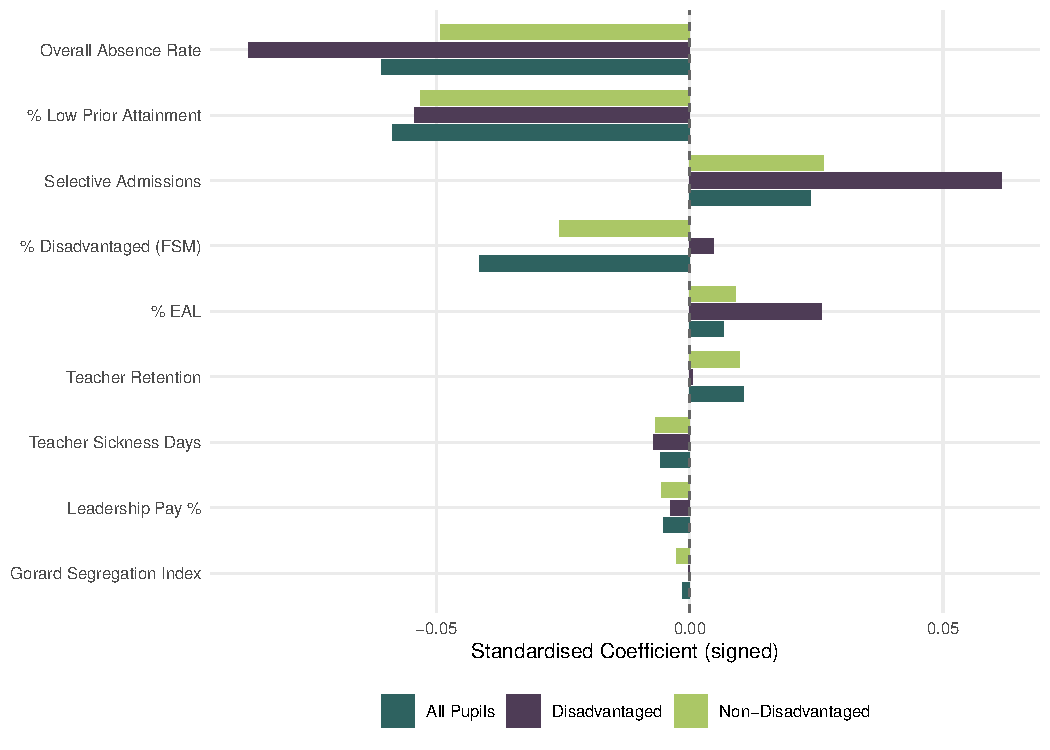
\includegraphics[keepaspectratio]{JEP_Paper_tight_files/figure-pdf/fig-standardised-coefficients-1.pdf}}

}

\caption{\label{fig-standardised-coefficients}Standardised coefficients
showing relative variable importance across pupil groups. Bars show the
change in log(ATT8) associated with a one-SD shift in each predictor.}

\end{figure}%

Figure~\ref{fig-standardised-coefficients} compares the standardised
coefficients\footnote{Standardised coefficients are computed as
  \(\beta^*_k = \hat{\beta}_k \times \text{SD}(x_k) / \text{SD}(\log \text{ATT8})\),
  where \(\text{SD}(x_k)\) is the sample standard deviation of the
  predictor (log-transformed where applicable). This rescales each
  coefficient to represent the change in outcome, in standard-deviation
  units, associated with a one-standard-deviation change in the
  predictor.} across all three pupil groups (all pupils, disadvantaged
pupils and non-disadvantaged pupils - full model outputs available in
the supplementary materials\footnote{Stepwise Models for all pupil
  groups
  \url{https://adamdennett.github.io/school_attainment_tool/model_results.html\#stepwise-model-building}}).
Absence is the dominant predictor across all groups, but it is
\emph{even more} important for disadvantaged pupils --- nearly half of
the variation in school-level performance for this group is explained by
attendance alone.

The most contentious finding in our analysis concerns concentrations of
disadvantage (contentious in Brighton and Hove - although the findings
echo the analysis of Macleod et al. (2015) a decade ago). For
non-disadvantaged pupils, higher FSM proportions are associated with
lower attainment. But for disadvantaged pupils, the coefficient is
\emph{positive} --- after controlling for absence and low prior
attainment, disadvantaged pupils perform slightly better in schools with
higher concentrations of other disadvantaged pupils. This finding is
robust across individual year models and alternative specifications of
disadvantaged attainment and disadvantage measures.\footnote{See
  supplementary material for robustness checks:
  \url{https://adamdennett.github.io/school_attainment_tool/model_experiments.html}}
In the full multilevel model, this positive coefficient shrinks
substantially, suggesting the effect operates through LEA-level and
Ofsted-level factors rather than concentration \emph{per se} --- schools
with higher FSM proportions in certain LEAs appear to have developed
effective support systems, possibly through targeted use of Pupil
Premium funding and other specialisations.

For non-disadvantaged pupils, the effects of higher disadvantage
concentrations are more clearly negative. Even after controlling for
attendance and prior scores, being in a higher-disadvantage school
depresses Attainment 8 for this group --- possibly due to a peer effect
or curriculum-resourcing dynamic. Both of these findings are contentious
in the Brighton and Hove context as they challenge the `no cost'
conjecture, but perhaps most importantly suggest that policy efforts to
make the schools in the city more mixed than they already are (Brighton
and Hove's schools are already in the top third for integration of
disadvantaged and non-disadvantaged students when using the Gorard
Segregation index\footnote{Gorard Segregation was calculated for all
  LEAs in 2022-23 and shown visually in this piece
  \url{https://adamdennett.github.io/BH_Schools_Consultation/absence.html\#trick-or-treatment}}
-- a fact that emerged during the 2024 consultation, but not one that on
its own moved the dial) might actually be counter productive as a policy
to improve disadvantaged attainment.

Absence remains consistently the biggest predictor across all groups and
is even more important for disadvantaged pupils. Nearly half of the
difference in school-level performance for disadvantaged pupils is
explained simply by whether they regularly attend. Disadvantaged pupils
may lack the safety net of engaged parents, private tutors or revision
resources that some less disadvantaged students have, which could be a
factor in making classroom instruction more important for them. In this
sense, attendance is the ultimate equity lever.

These outcomes do not advocate for concentrating disadvantaged pupils.
We do not. However, where the social and spatial composition of LEAs
means that disadvantaged and non-disadvantaged students are not evenly
spread across schools, deconcentration policies premised on the
assumption that disadvantaged pupils inevitably fare worse in schools
with lower concentrations of disadvantage are not supported by this
evidence. And where remediating policies require longer journeys that
risk increasing absence (Thomson 2023), they could be actively
counter-productive given how much more negatively impactful absence is.

\section{Brighton and Hove case
study}\label{brighton-and-hove-case-study}

\subsection{Local context}\label{local-context}

Brighton and Hove has ten secondary schools: six community schools run
by the LEA, two academies (Brighton Aldridge Community Academy --- BACA
--- and Portslade Aldridge Community Academy --- PACA) and two church
schools (King's and Cardinal Newman) that set their own admissions.
Following the closure of CoMArt in the east of the city in 2005, large
catchment areas were introduced (Figure~\ref{fig-catchments}) with a
lottery tie-break for oversubscribed schools --- making admissions very
different to most other places in England where distance typically
determines priority (Allen et al. 2013).

In October 2024, the council launched proposals to amend the secondary
school admissions process with the intention of improving disadvantaged
attainment. The proposals were to reduce Published Admission Numbers at
popular central schools, redraw catchment boundaries, and reserve 20\%
of places in some schools for out-of-catchment children. The stated aims
were to improve educational outcomes for disadvantaged pupils and ensure
financial viability of under-subscribed schools located at the
geographic periphery of the city. Underpinning the proposals was an
assertion that attainment in the city was `driven by economic advantage'
(e.g.~housing costs near better performing schools --- a common
misconception empirically disproven in the Brighton and Hove context by
Tan and Dennett (2025)) and that redistributing disadvantaged pupils
would narrow the attainment gap, drawing on the work of Gorard and
Siddiqui (2019) on school segregation. This built on a 2023 policy
giving FSM-eligible pupils priority in admissions at schools with below
the city-average (30\%) FSM share, which was already producing flows
from peripheral to more popular central catchments.

The public response was overwhelmingly negative, with the council's
feedback summary from the pre-consultation engagement exercise noting
\emph{`a strong preference for improving existing schools rather than
redistributing students, alongside deep concerns about potential impacts
on community cohesion and student wellbeing'}. The proposals would, by
the council's own calculations, force significant numbers of children
from central catchments to attend schools at the periphery of the city,
potentially requiring over two hours of daily school commuting for many
pupils. To support these increased flows, the council also signalled
additional bus provision to ferry children between catchments, with the
associated transport costs (running into hundreds of thousands of pounds
annually for a single route) absorbed by the council.

Whether the availability of better evidence would have changed the
political outcome is unknowable. But with lived experience of responding
to the council's proposals, we can say that accessible evidence
\emph{would} have enabled earlier and more constructive engagement.
Without ease of data access, the compressed consultation timeline left
inadequate time to assemble and present counter-evidence for the
complexity of the issues at stake. What follows is an attempt to
demonstrate what that evidence looks like.

\begin{figure}

\centering{

\pandocbounded{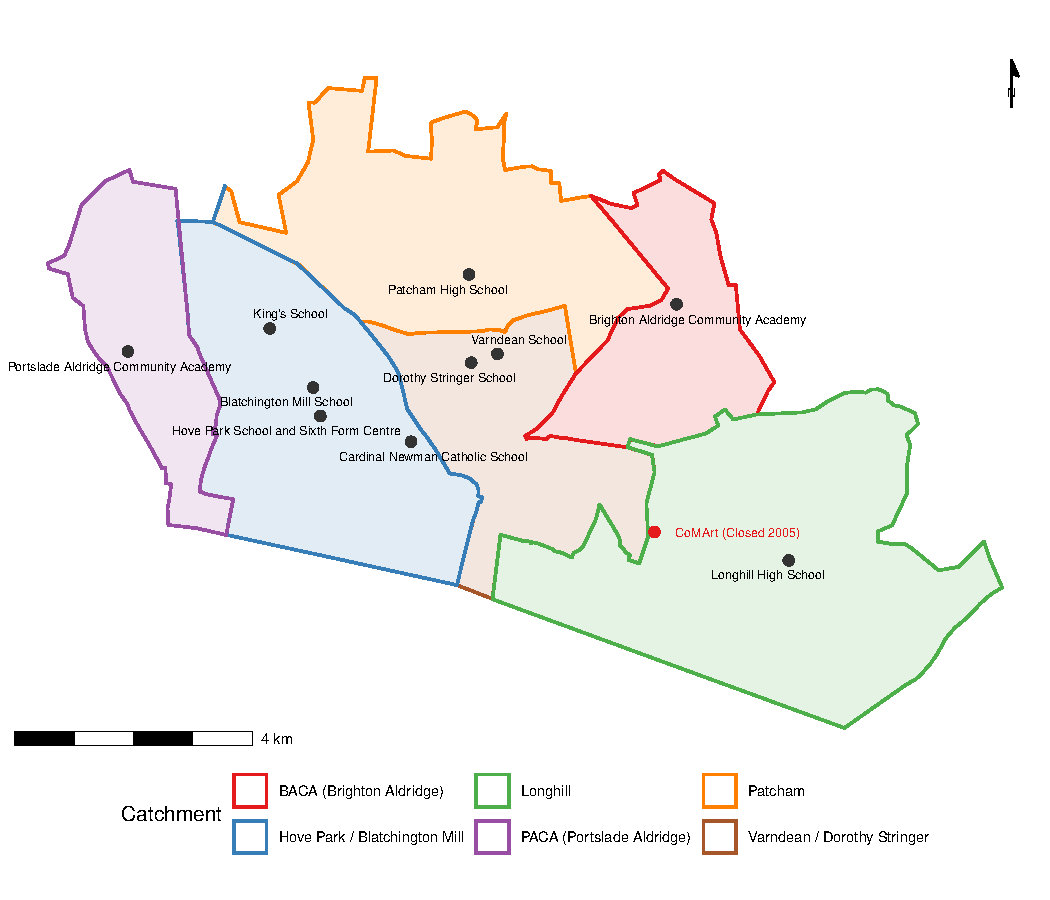
\includegraphics[keepaspectratio]{JEP_Paper_tight_files/figure-pdf/fig-catchments-1.pdf}}

}

\caption{\label{fig-catchments}Brighton and Hove secondary schools with
2025/26 catchment boundaries.}

\end{figure}%

\subsection{Local authority effects}\label{local-authority-effects}

\begin{figure}

\centering{

\pandocbounded{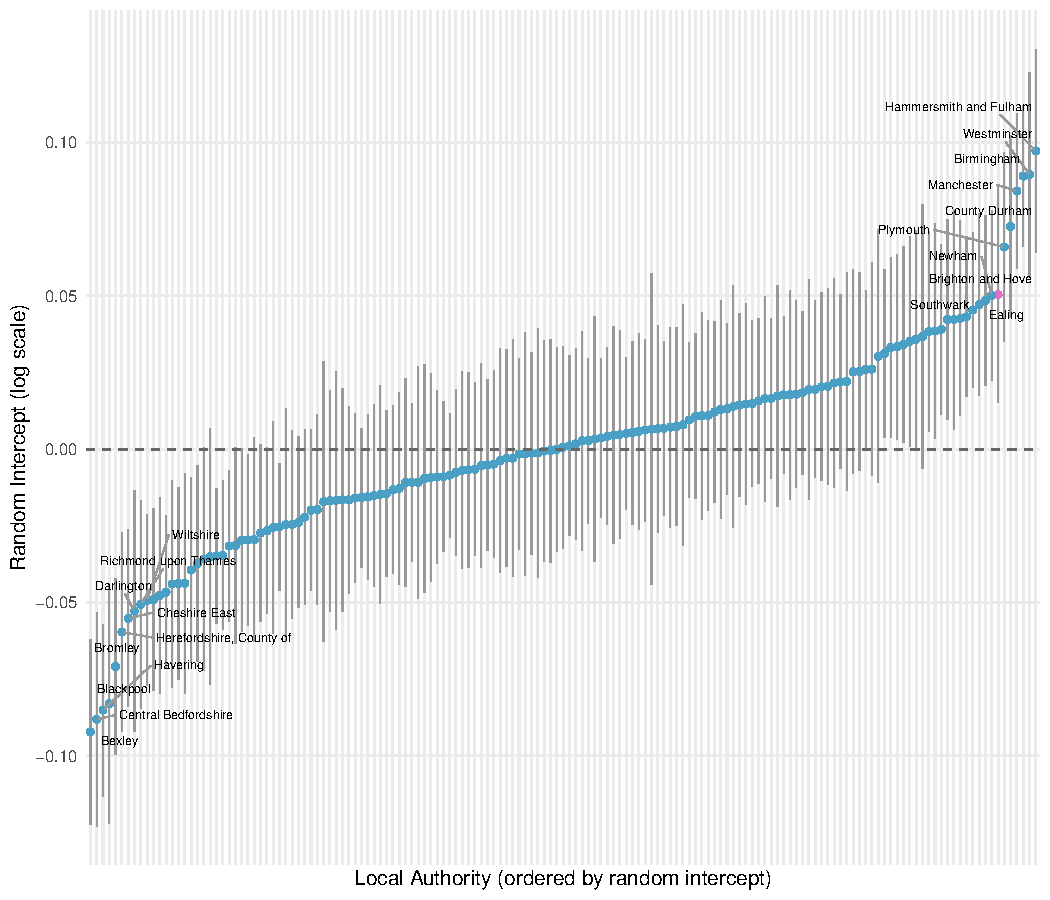
\includegraphics[keepaspectratio]{JEP_Paper_tight_files/figure-pdf/fig-caterpillar-1.pdf}}

}

\caption{\label{fig-caterpillar}LA random intercepts for
disadvantaged-pupil attainment (imputed full panel model). Top and
bottom 10 LAs labelled; Brighton and Hove highlighted.}

\end{figure}%

Figure~\ref{fig-caterpillar} shows that Brighton and Hove ranks 7th out
of 152 LEAs for disadvantaged attainment once structural factors are
accounted for in the multilevel model presented earlier. For
non-disadvantaged pupils it ranks 5th; for all pupils, 4th. The positive
random intercept of approximately +0.06 translates to around a 6\%
uplift in Attainment 8 --- roughly 2 GCSE points above what structural
factors would predict. This was unknown at the time of the 2024
consultation and entirely absent from the public narrative, which was
framed around a premise of failure, based on limited analysis.

\subsection{Comparing policy levers: absence versus
disadvantage}\label{comparing-policy-levers-absence-versus-disadvantage}

Because the model uses log-transformed variables, the same
percentage-point change produces different effects depending on where a
school starts --- returns \emph{accelerate} as values improve.
Figure~\ref{fig-accelerating-returns} places both the absence and FSM
levers on a common y-axis.

\begin{figure}

\centering{

\pandocbounded{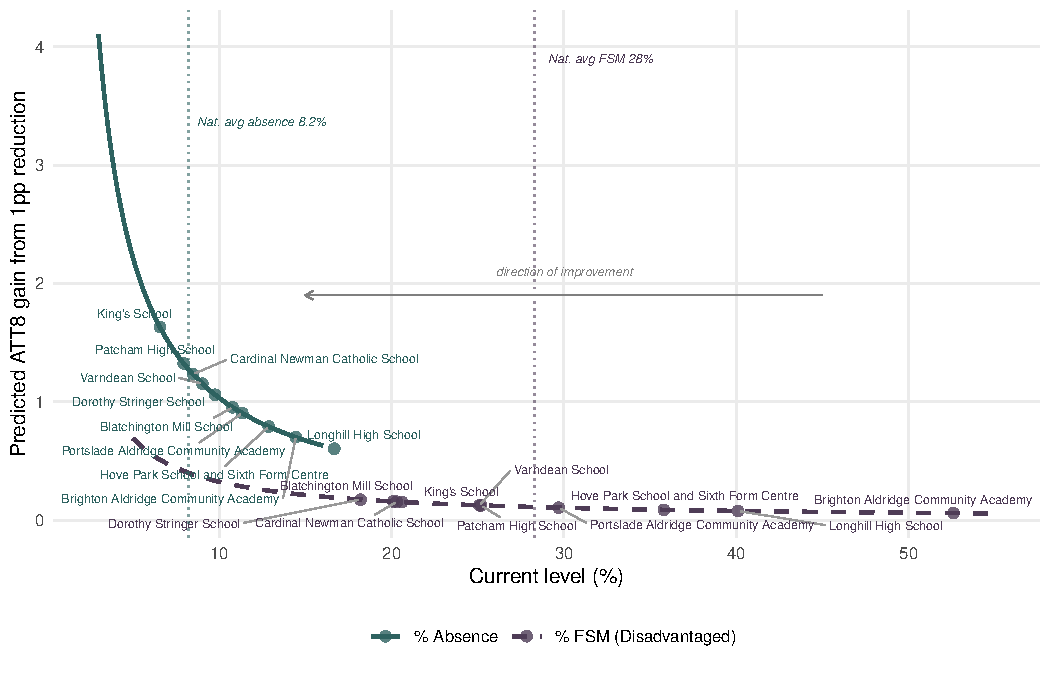
\includegraphics[keepaspectratio]{JEP_Paper_tight_files/figure-pdf/fig-accelerating-returns-1.pdf}}

}

\caption{\label{fig-accelerating-returns}Accelerating returns: each
percentage-point reduction buys a progressively larger ATT8 gain
(reading right to left). Absence delivers substantially larger gains
than FSM at every level. Brighton and Hove schools marked on each
curve.}

\end{figure}%

Three features are immediately visible. First, the absence curve sits
above the FSM curve at every starting level. Second, the gap
\emph{widens} as values improve. Third, Brighton and Hove schools
cluster in the flatter right-hand portion for both variables, but the
city's position is far more extreme for absence.

Brighton and Hove's mean school FSM rate (28.8\%) is close to the
national average (28.3\%). But the city's mean absence rate (10.8\%)
against a national average of 8.2\% places it at the 99th percentile ---
among the very worst in England. When standardised by the city's spread,
the absence coefficient is 2.6 times as important as FSM for predicting
attainment.

Bringing schools above the national average for absence down to it would
produce predicted gains averaging +2.9 Attainment 8 points per school,
with gains for disadvantaged pupils averaging +3.3 points. Even dramatic
FSM reductions would yield gains closer to 1 point. On the evidence,
attendance is the single most consequential lever the city has
available, and admissions changes of the kind proposed in 2024 are very
unlikely to produce equivalent gains in disadvantaged attainment.

\subsection{Contextualised school
performance}\label{contextualised-school-performance}

\begin{figure}

\centering{

\pandocbounded{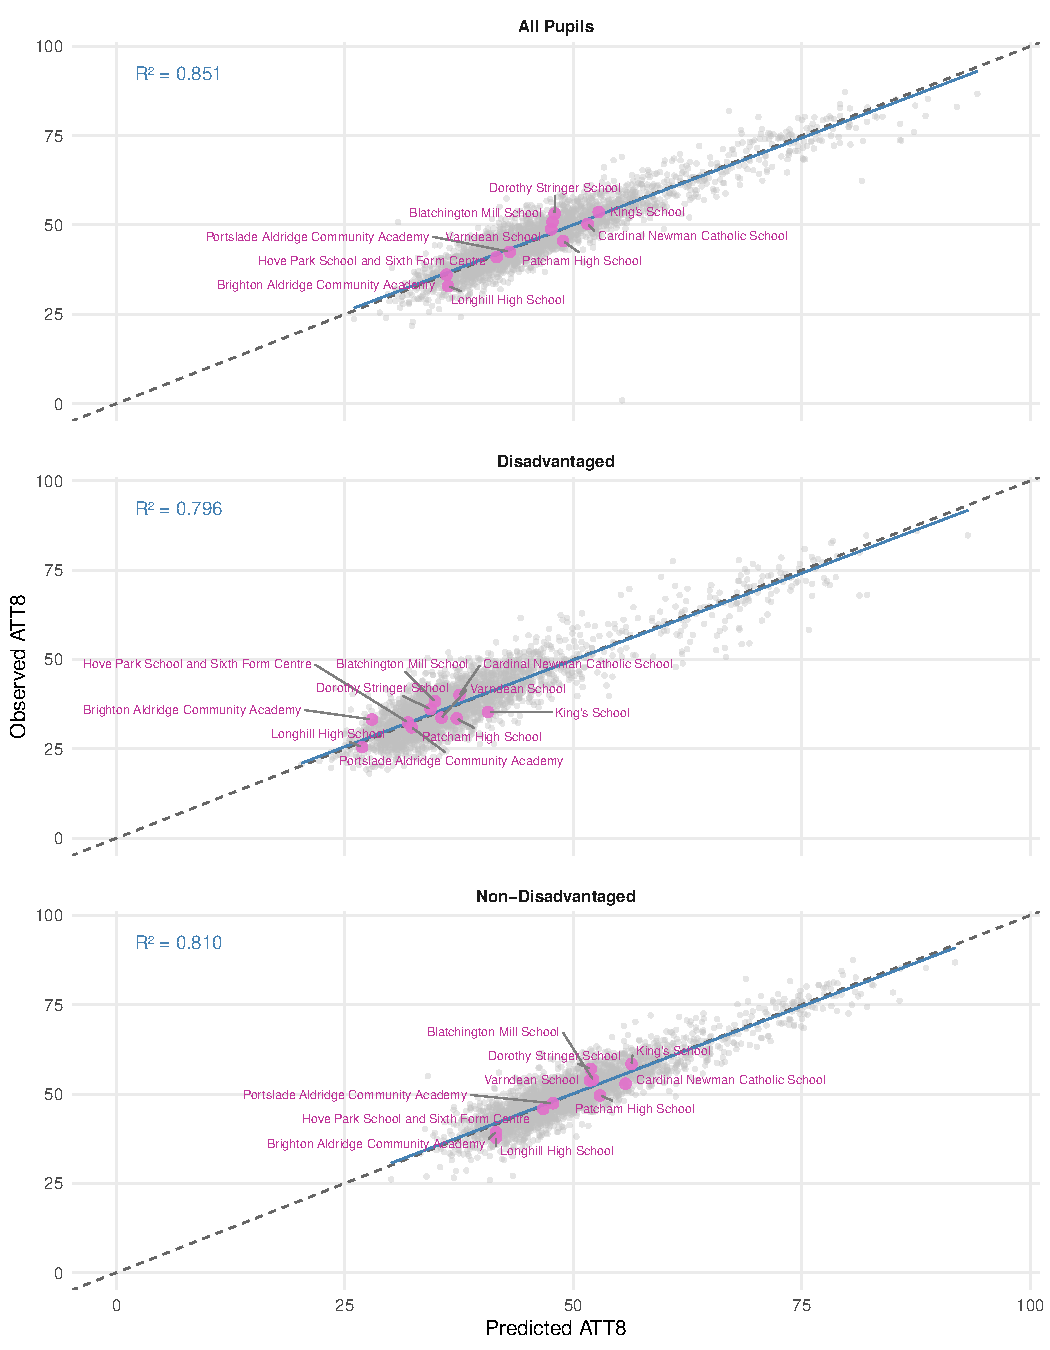
\includegraphics[keepaspectratio]{JEP_Paper_tight_files/figure-pdf/fig-obs-vs-pred-1.pdf}}

}

\caption{\label{fig-obs-vs-pred}Observed versus predicted Attainment 8
for Brighton and Hove schools (highlighted) against all schools
nationally, 2024--25.}

\end{figure}%

Figure~\ref{fig-obs-vs-pred} shows observed versus predicted Attainment
8 for the latest year across all schools in England (grey) with Brighton
and Hove schools highlighted (pink). The close clustering of the points
around the diagonal line is a visual representation of the \(R^2\)
values show on the plot and in the tabular model outputs shown earlier -
observed values for most schools are close to the model predictions. The
model residuals --- the vertical distance from the diagonal --- show
whether a school is doing better (above) or worse (below) than the model
predicts and provides what we might think of as contextualised
`value-added' measures - more nuanced than Progress 8 - as this
model-based value added accounts for far more than just prior attainment
in its representation.

\subsection{Decomposing absence: structural intake versus school
management}\label{decomposing-absence-structural-intake-versus-school-management}

The contextualised value-added reading above hides a complication we
should make explicit. Our headline model treats school-level absence as
a single regressor on the same footing as the school's other intake
variables, but absence is a little differnt to deprivation or English as
and additional language. Some of school-level absence is exogenous to
the school: driven by family circumstances, area-level health trends,
deprivation patterns, the SEND profile of the catchment and other
features of the intake the school inherits but cannot directly choose.
However some of it is produced by the school: through pastoral systems,
attendance officers, parental engagement and the broader ethos around
getting children into class. When we control for raw absence in our
headline model, both components are absorbed together --- the
school-level residual we have just been calling `value-added' reflects
what the school does \emph{given} its attendance, not what it does
\emph{to} its attendance.

However, it is possible to separate these endogenous and exogenous
elements of absence via A two-stage decomposition\footnote{Full
  technical details, model fits, sensitivity checks and a 50-replicate
  clustered bootstrap of school rank uncertainty are in the
  supplementary material:
  \url{https://adamdennett.github.io/school_attainment_tool/model_experiments.html\#sec-two-stage-absence}}.
Firstly, we fit a new absence model in which school-level absence is
modelled only on the variables we treat as exogenous to the school (FSM,
EAL, low prior attainment, segregation, plus place and year random
effects). This produces two derived quantities for every school-year: an
\emph{expected absence} (the part the intake predicts) and a
\emph{residual absence} (what is left over --- broadly, the
school-controllable component). Secondly, we refit the attainment model
with the intake-predicted absence in place of raw absence, and we drop
the workforce predictors. The school-level residual from this refitted
attainment model is a more honest value-added measure: it gives credit
for what the school adds to attainment over and above its intake,
\emph{with} attendance management already counted as part of the
school's contribution rather than stripped away as a control.

The national-level picture this paints is informative. Most of the
school-year variation in absence is explained by the intake-only first
stage --- absence at school level is dominated by intake and place-level
structural factors. The school-controllable residual is the smaller
share, and a model that fits expected absence and residual absence as
separate predictors confirms that the marginal contribution of residual
absence to attainment is modest at England school level once
intake-driven absence is already accounted for. This does not mean
attendance management is unimportant. It means the headline raw-absence
coefficient borrows much of its statistical force from the structural
component. The lever is real, but the school-only portion of it is
smaller than the single coefficient implies. For local education
authorities this has direct policy consequences: closing a city's
absence problem requires both school-level attention \emph{and}
cross-departmental work --- public health, children's services,
area-level deprivation policy --- because much of what schools are
dealing with on attendance is inherited from within the LEA, rather than
generated.

\begin{figure}

\centering{

\pandocbounded{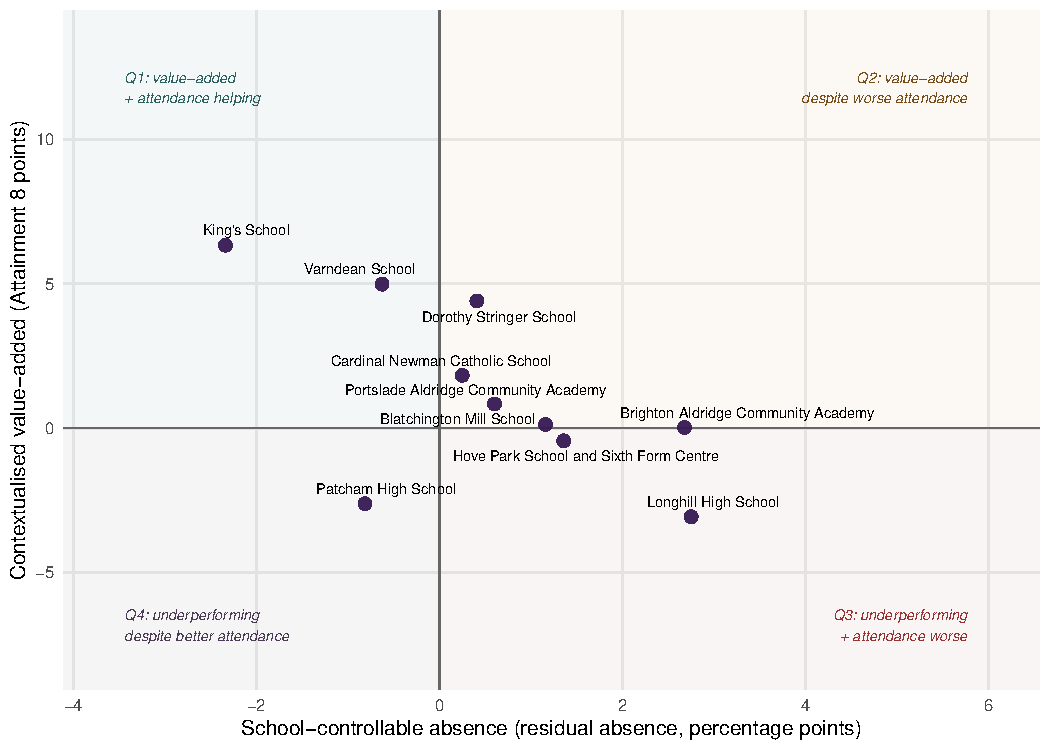
\includegraphics[keepaspectratio]{JEP_Paper_tight_files/figure-pdf/fig-quadrant-1.pdf}}

}

\caption{\label{fig-quadrant}Brighton and Hove secondaries on the
joint-signal plane: contextualised value-added (vertical, in Attainment
8 points) versus the school-controllable absence component (horizontal,
in percentage points). The reference lines at zero on each axis split
the plane into four narrative quadrants discussed in the text. The full
national version with a local-authority filter is available
interactively in the project's HTML report.}

\end{figure}%

For local school-level diagnostics the decomposition becomes
considerably more informative. Two signals can now be read side by side:
the school's contextualised value-added, and its residual absence
(positive when the school runs more absence than its intake would
predict, negative when less). Sorted on these two axes
(Figure~\ref{fig-quadrant}), schools fall into four meaningful policy
stories: schools adding value with attendance management helping (Q1,
top-left); schools adding value despite worse-than-predicted attendance
(Q2, top-right); schools underperforming with attendance the cleanest
single lever (Q3, bottom-right); and schools underperforming despite
unusually good attendance management (Q4, bottom-left).

For Brighton and Hove the joint-signal view sharpens the case-study
reading. Most of the city's schools sit in Q2 in the top-right: they are
delivering attainment above what their intake would predict and is doing
so while running more absence than their intake-driven absence model
expects. In these schools, the pedagogical work happening is the more
impressive for it; closing any of these school's residual-absence gap
would compound directly onto an already-strong value-added signal. Any
schools in Q4 provide a challenge: their attendance management is
genuinely strong, but once intake is properly accounted for their
attainment outcomes fall short of what their profile predicts, so the
simple ``fix attendance'' improvement story is not available. Schools in
Q3 are the most natural targets for council-led attendance
interventions, and Q1 schools are where the city should look for
practice worth sharing. Reporting \textbf{value-added alongside residual
absence}, with explicit uncertainty intervals, is a more honest framing
than the single number that conventional benchmarking produces, and
would help align local policy conversation with what the data can
support.

\section{Discussion}\label{discussion}

\subsection{The danger of single-lever policy
thinking}\label{the-danger-of-single-lever-policy-thinking}

The Brighton and Hove experience illustrates the risks of building a
policy around a single causal narrative. The council's 2024 admissions
proposals were built around the premise that redistributing
disadvantaged pupils would narrow the attainment gap. In the
consultation papers released to the public\footnote{Brighton and Hove
  Council 2024 Consultation Papers:
  \url{https://yourvoice.brighton-hove.gov.uk/en-GB/projects/school-admission-arrangements-public-consultation/1}},
it was stated:

\begin{quote}
\emph{``We also know that children from disadvantaged homes are less
likely to do well at school and that can be made worse when more
disadvantaged children all go to school together. We are looking at
options for how we can help the city manage that issue better, including
through our school admissions arrangements.''}
\end{quote}

This premise sits awkwardly with the existing evidence base. Macleod et
al. (2015)'s earlier analysis for the DfE found that, controlling for
intake characteristics, schools with higher concentrations of
disadvantage tend to do \emph{better} for their disadvantaged pupils,
not worse. Our more up-to-date modelling on four years of national data
reaches the same conclusion. Concentrations of disadvantage are one of
the weaker available levers, and for disadvantaged pupils specifically
the direction of the effect runs in the opposite direction to the policy
assumption. The implication is that admissions changes of the kind
proposed in Brighton and Hove are unlikely to deliver the targeted gains
in disadvantaged attainment.

The chosen lever also carries its own risks that the proposals did not
engage with. Redistribution policies necessarily generate longer
journeys to school for many pupils, and the wider literature is clear
that long commutes are associated with reduced sleep and its
psychosocial (Fredriksen et al. 2004; Yeo et al. 2019), physical
(Voulgaris et al. 2019; Pradhan and Sinha 2017; Pereira et al. 2014;
Faulkner et al. 2013) and mental health (Nakajima et al. 2024;
Chairassamee et al. 2024; Guan et al. 2025) consequences, including
stress (Karan et al. 2021) and general wellbeing (Ding et al. 2023), and
crucially with \emph{higher absence} across multiple national settings
(Otsuka et al. 2025; Cordes et al. 2022; Blagg et al. 2018), including
England (Thomson 2023). Absence is the single largest predictor of
attainment in our modelling and the city's most acute structural
problem; a policy that even marginally increases it could be
counterproductive in attainment terms. The claim that social mixing can
be achieved at `almost no cost' (Gorard and Siddiqui 2019) does not
survive contact with this second-order literature.

There is a further, more qualitative dimension to displacing pupils from
their local schools. Schools serve as community anchors for the families
and neighbourhoods around them: walked-to schools, friendship groups
that map onto local catchments, parental engagement that depends on
geographic proximity, and active travel that supports physical and
mental health (Faulkner et al. 2013). A masters-level case study of
extended commutes in Chicago (Shah 2023) argues that the burden of long
commutes falls disproportionately on pupils already experiencing other
forms of marginalisation. Long-distance transit also predicts early high
school transfer (Stein et al. 2021), itself a known risk factor for poor
attainment. These are not peripheral concerns; they are part of the
cost-benefit calculus that any redistribution policy needs to take
seriously, and they were largely missing from the 2024 deliberation.

\subsection{Attendance as the most impactful single
lever}\label{attendance-as-the-most-impactful-single-lever}

A policy conversation about Brighton and Hove's disadvantage attainment
gap that wants to make the largest predictable difference should put
\textbf{attendance} at its centre. The city has the second-worst absence
rate in England, and the wider evidence indicates that closing this gap
would yield attainment gains for disadvantaged pupils that comfortably
exceed anything achievable through changes to admissions arrangements
--- and would do so \emph{without} the social, health and travel costs
that a redistribution-led approach implies.

Brighton and Hove's absence rates are not a necessary consequence of its
intake composition. The city has near-average FSM eligibility levels but
near-worst absence, suggesting the problem reflects local factors ---
attendance culture, enforcement practices, transport friction or
community dynamics --- rather than being an unavoidable correlate of
disadvantage. If the city is not already running a substantial
cross-departmental attendance programme alongside its school-level work,
the case for one is strong. There is also a budget question here that
policy makers may want to weigh transparently: the additional bus
provision required to support the proposed catchment changes is itself a
non-trivial cost, and resources of that scale invested directly in
attendance support, family liaison and pastoral capacity in the city's
most affected schools would have a stronger evidence base for raising
disadvantaged attainment than the same money spent on transport that
reduces children's time outside of school.

\subsection{A new value-added view to support better local
decisions}\label{a-new-value-added-view-to-support-better-local-decisions}

A second contribution of this work is methodological. The multilevel
model lets us look beyond a school's raw attainment outcomes and ask how
much it is adding \emph{over and above} the structural intake
characteristics it inherits --- characteristics that the school cannot
itself choose. The school-level random intercept, plus the school-level
residual from the fitted model, gives us a contextualised value-added
view that is fairer than the headline attainment number and more
informative than a single-word Ofsted rating, both for parents making
school choices and for policy makers assessing where local effort is
best directed. Brighton and Hove provides a particularly sharp
illustration of why this matters: the local school for one of the city's
most disadvantaged catchments is, on this view, doing materially better
for its disadvantaged pupils than the schools to which a number of those
pupils' families have been opting to travel.

\begin{table}

\caption{\label{tbl-league}Value-added rankings for Brighton and Hove
schools (panel model residuals by year, in Attainment 8 points).}

\centering{

\centering\begingroup\fontsize{8}{10}\selectfont

\resizebox{\ifdim\width>\linewidth\linewidth\else\width\fi}{!}{
\begin{tabular}[t]{rlrrrr>{}r}
\toprule
Rank & School & 2021-22 & 2022-23 & 2023-24 & 2024-25 & Mean\\
\midrule
\addlinespace[0.3em]
\hline
\multicolumn{7}{l}{\textit{\textbf{All Pupils}}}\\
\hspace{1em}1 & Dorothy Stringer School & +3.5 & +3.8 & +2.8 & +5.2 & \textbf{+3.8}\\
\hspace{1em}2 & Varndean School & +4.0 & +3.3 & +6.0 & +1.2 & \textbf{+3.6}\\
\hspace{1em}3 & King's School & +4.8 & +0.1 & +5.9 & +0.8 & \textbf{+2.9}\\
\hspace{1em}4 & Portslade Aldridge Community Academy & +2.9 & -0.4 & +3.1 & -0.5 & \textbf{+1.3}\\
\hspace{1em}5 & Brighton Aldridge Community Academy & +2.0 & +1.2 & +0.4 & -0.0 & \textbf{+0.9}\\
\hspace{1em}6 & Blatchington Mill School & -2.2 & -0.8 & +2.5 & +3.1 & \textbf{+0.6}\\
\hspace{1em}7 & Hove Park School and Sixth Form Centre & +0.6 & +2.0 & +0.4 & -0.6 & \textbf{+0.6}\\
\hspace{1em}8 & Cardinal Newman Catholic School & +0.4 & -1.7 & +1.2 & -1.3 & \textbf{-0.3}\\
\hspace{1em}9 & Longhill High School & +0.4 & -2.2 & -2.2 & -3.4 & \textbf{-1.8}\\
\hspace{1em}10 & Patcham High School & -3.2 & -2.7 & -4.9 & -3.4 & \textbf{-3.6}\\
\addlinespace[0.3em]
\hline
\multicolumn{7}{l}{\textit{\textbf{Disadvantaged Pupils}}}\\
\hspace{1em}1 & Brighton Aldridge Community Academy & +3.2 & -1.3 & +4.1 & +5.2 & \textbf{+2.8}\\
\hspace{1em}2 & Varndean School & +3.2 & +3.6 & +4.5 & -1.9 & \textbf{+2.3}\\
\hspace{1em}3 & Dorothy Stringer School & +2.9 & +3.2 & +0.3 & +1.7 & \textbf{+2.0}\\
\hspace{1em}4 & Cardinal Newman Catholic School & +2.4 & -5.0 & +6.5 & +2.5 & \textbf{+1.6}\\
\hspace{1em}5 & King's School & +5.8 & +0.9 & +4.4 & -5.4 & \textbf{+1.5}\\
\hspace{1em}6 & Blatchington Mill School & -5.4 & +1.3 & +5.2 & +3.4 & \textbf{+1.1}\\
\hspace{1em}7 & Hove Park School and Sixth Form Centre & +2.4 & -1.7 & +1.3 & +0.5 & \textbf{+0.6}\\
\hspace{1em}8 & Portslade Aldridge Community Academy & +2.6 & -4.0 & +4.7 & -1.3 & \textbf{+0.5}\\
\hspace{1em}9 & Patcham High School & +3.8 & +1.6 & -11.9 & -3.7 & \textbf{-2.6}\\
\hspace{1em}10 & Longhill High School & -4.6 & -6.2 & +0.8 & -1.4 & \textbf{-2.9}\\
\bottomrule
\end{tabular}}
\endgroup{}

}

\end{table}%

In the period of the 2024 consultation the public debate in the city
shifted slightly, away from how the council's proposals were going to
improve disadvantaged attainment to how they were facilitating parental
choice. Choice in this instance was largely to do with parents
perceiving their local options to be poor and wanting access to
alternatives. An activist group (Equity in Education\footnote{\url{https://educationequity.kit.com/}}
--- supported by another more established activist group --- Class
Divide\footnote{\url{https://www.classdivide.co.uk/}}) emerged from
within the BACA catchment advocating for parents to have more options
available to \emph{not} send their children to that school. At the time
BACAs Ofsted rating was `requires improvement' and its raw attainment
scores were some of the lowest in the city --- creating an impression of
that school being a poor option.

As a family deciding on where to send their child, they can decide based
on how the school performs overall, or where a school increases
attainment beyond the structural disadvantage faced by their pupils
(over which they have little control). These do not always lead to the
same answer. In Brighton and Hove, one of the outcomes that emerged from
the vocal public debate, was a considerable number of parents from the
BACA catchment opting to send their children to Patcham School (in the
neighbouring catchment --- see Figure~\ref{fig-catchments}) for entry in
2025 and 2026 --- a school rated `Good' by Ofsted and with raw
attainment scores placing somewhere mid-table in the city. However, if
we move beyond the raw attainment scores and blunt single-word Ofsted
ratings, a very different picture of the two schools emerges. BACA is
situated in one of the most economically deprived parts of Brighton and
Hove, Patcham, one of the more economically prosperous. BACAs absence
rates have been in excess of the very high city average. Patcham is one
of two schools in the City with absence rates below the national
average. The number of pupils entitled to Free School Meals attending
BACA is around 50\%, at Patcham it is around 25\%. Around 30\% of the
pupils attending BACA have low prior attainment, at Patcham it is around
16\%. When we account for these stark cohort differences in our model, a
very different picture of school effectiveness occurs.

These are, of course, school-level observations and difficult to
translate into predictions about whether Pupil A will be better-off
attending school X or school Y, but they do correspond to an average
expected situation. As the league tables in Table~\ref{tbl-league},
derived from Figure~\ref{fig-obs-vs-pred} in above reveal, in 2024-25, a
disadvantaged pupil attending BACA and taking their GSCEs would have, on
average, left that school with GCSEs 5-points higher than if they'd
attended a similar school with a similar profile elsewhere in England.
Over the last 4 years, this would have averaged around 3 points higher.
This is a boost way in excess of the fraction of a point differences
that might be expected from altering the disadvantage mix in schools.
BACA is doing incredibly well for its disadvantaged students and indeed
out-performs every other school in the city by some margin --- even
those which in the popular imagination are viewed as the `best' or most
desirable schools in the city, e.g.~Varndean, Cardinal Newman. BACA in
some ways is the case study that illuminates the findings in the
national data earlier in this paper which showed that disadvantaged
attainment is higher in schools with bigger concentrations of
disadvantaged students and in direct contradiction to the statement in
Brighton and Hove City Council's consultation materials. In April 2025,
BACA received a new Ofsted report which rated it `Good' in all 5 areas
of provision\footnote{\url{https://reports.ofsted.gov.uk/provider/23/136164}}
--- a result unsurprising in the context of this data analysis, but
probably more surprising to anyone just looking at raw prior attainment
and previous Ofsted report.

If we contrast BACA --- the school popular narrative discouraged parents
from sending their children to --- with Patcham --- the school many from
BACA catchment in the end opted for, the differences on this alternative
league table are stark. Disadvantaged pupils attending Patcham on
average over the last 4 years and compared to other disadvantaged pupils
attending schools with similar profiles elsewhere in England, would
leave with around 2.6 GCSE points fewer than they might be expected to
compared to similar schools elsewhere in England. In 2023-24, the
difference was in double figures. These differences have been hidden
from view amongst the comfortable mid-table position, in raw attainment
terms, the school has enjoyed. There might be many reasons why parents
would want to opt for Patcham High School over BACA - some may
reasonably ask why it would be better to send a child to a school doing
well ``considering'' vs doing well in raw terms? The answer is that at
the school-level, those statistics reflect ALL children (including all
of those who, for example, missed a lot of school and consequently did
poorly in their exams). The ``considering'' element of this analysis and
the nuance nuance it affords to the effectiveness of these schools by
showing the value added in the face of (in our example) high levels of
absence, reveals the underlying positive features of the school that
will benefit all pupils. The modelling in this paper helps provide this
alternative view that might have made some of parents from BACA
catchment who opted to send their children to Patcham, make a different
decision.

One thing other schools in the city certainly could learn from Patcham
High School is in how to improve attendance rates. The school is one of
only two in the city with attendance better than the national average.
This is an actionable policy lever at the school-level. Without a deeper
dive into attendance issues at the different schools in the city, it's
impossible to know what the drivers of this issue are. But given we now
know where the real problems in Brighton and Hove lie at the LEA level,
one useful policy focus at the city level could well be exploring how
schools like Patcham are able to keep attendance relatively high, while
then allowing more school-level investigations into where
under-performance might be occurring given our new knowledge of
interacting structural drivers within the city.

\subsection{Viability versus
attainment}\label{viability-versus-attainment}

The 2024 consultation papers stated two aims: improving disadvantaged
attainment, and ensuring the financial viability of under-subscribed
schools at the city's periphery. Since schools are funded on a per-pupil
basis, financial viability is a legitimate concern, particularly given
the historical context of an earlier school closure in a deprived part
of the city that left some pupils already travelling long distances to
peripheral provision. There is, however, an inherent tension between
optimising for financial sustainability and optimising for educational
outcomes. The two cases need to be weighed transparently. The
contextualised value-added view introduced above suggests that the
city's pattern of school-level effectiveness does not map cleanly onto
raw attainment or popularity: if redistribution moves children from
schools adding more value to schools adding less, the aggregate impact
on city-wide attainment could be negative even if the financial case for
the receiving schools improves.

Following widespread opposition and appeals to the Schools Adjudicator,
the proposed PAN reductions were rejected and the 20\% out-of-catchment
priority was reduced to 5\%. While displacement was minimised, the
policy reverberations continued through choices expressed by parents
already influenced by the preceding debate.

\subsection{What is driving Brighton and Hove's over-achievement? And
what we don't yet
know}\label{what-is-driving-brighton-and-hoves-over-achievement-and-what-we-dont-yet-know}

The LEA random effect for Brighton and Hove is large and statistically
significant across all three attainment groups. After accounting for the
structural (disadvantage, absence, prior attainment) or school
management and governance (workforce characteristics, staff retention)
factors in the model - schools in the city consistently outperform what
the national picture would predict. For disadvantaged pupils, the city
ranks 7th; for non-disadvantaged pupils, 5th; for all pupils, 4th in
England.

This is a genuinely important finding that should re-frame the policy
conversation. The starting point for the 2024 consultation was a
narrative of failure --- the city was presented as uniquely failing its
disadvantaged students, sitting on a vast attainment gap, with radical
structural reform required to address the problem. The evidence suggests
the opposite: Brighton and Hove is one of the highest-performing LEAs in
the country once we account for the factors that we know drive
attainment. Rather than asking what the city is doing wrong, the more
productive question is what it is doing right --- and how that can be
protected and extended?

The honest answer is that we do not yet know what produces this LEA
effect. The random effect, by definition, captures variance that the
fixed-effect predictors do not explain. It could reflect high levels of
parental engagement and aspiration --- Brighton and Hove has a
well-educated population with a strong civic culture. It could relate to
the quality of school leadership and governance across the city, or to
effective local authority support services and school improvement
programmes. It could be something about the collaborative relationships
between schools, or community factors that are difficult to quantify.
Identifying the sources of this over-performance is an important
research question in its own right, and one that could require
additional qualitative investigation or access to pupil-level data that
goes beyond what is publicly available. What is clear, however, is that
policy interventions which risk disrupting a well-functioning system
without understanding what makes it function well carry substantial
downside risk.

\subsection{Implications for national
policy}\label{implications-for-national-policy}

The DfE (2026) white paper's ambitions will founder if pursued at the
local level without adequate analytical infrastructure. Every LEA
occupies different positions along the non-linear curves that relate
predictors to outcomes. What works in one context may be
counterproductive in another. The DfE's open data provides most of the
raw materials, but there is a crucial gap between raw data availability
and the accessible, contextualised intelligence that decision makers
need.

We have developed an interactive Policy Simulator tool,\footnote{School
  Attainment Policy Simulator:
  \url{https://adam-dennett.shinyapps.io/School_Attainment_Policy_Simulator/}}
underpinned by the models in this paper, to begin bridging that gap. The
tool allows users to explore any school in England, compare against
contextual expectations, and model the indicative impact of changes to
key variables.

\subsection{Limitations}\label{limitations}

These are school-level models built from aggregate published data, not
pupil-level analyses. The associations identified are not experimental
causal estimates but the best approximations available from
observational data. The models cannot capture unmeasured factors such as
school culture, parental engagement, or individual pupil resilience. The
Policy Simulator translates associations into indicative, not
definitive, projections. We do not claim that reducing absence by a
given amount will mechanically produce the predicted gain --- the real
world is more complex than any model captures. What we do claim is that
these models are accurate enough, and the patterns consistent enough
across years and specifications, to substantially improve the quality of
the conversation around what matters most.

\section{Conclusion}\label{conclusion}

This paper has demonstrated that the DfE's open data is a substantially
underutilised resource for understanding school attainment. School-level
Attainment 8 is remarkably predictable from a small number of variables,
and that predictability creates opportunities for better-informed local
policy. The Brighton and Hove case study yields three positions we feel
are well-supported by the evidence presented here.

First, the city's 2024 admissions proposals were built on a premise ---
that concentrations of disadvantage are a primary driver of low
disadvantaged attainment --- that does not survive contact with the four
years of national data analysed here, nor with the earlier
DfE-commissioned analysis (Macleod et al. 2015). Combined with the wider
literature on the consequences of long school commutes for sleep,
health, wellbeing, attendance, school transfer and the loss of
community-anchored schooling, the proposals are unlikely to deliver the
targeted gains in disadvantaged attainment and carry a set of social and
educational costs that the consultation did not engage with.

Second, the single most consequential lever available to Brighton and
Hove for raising disadvantaged attainment is \textbf{attendance}. The
city has the second-worst absence rate in England, and the modelling
suggests that moving the city's worst-affected schools toward the
national absence average would yield gains for disadvantaged pupils that
comfortably exceed anything achievable through admissions reform. If the
city is not already running a substantial cross-departmental attendance
programme, the case for one is strong; resources of the scale required
to bus children between catchments would, on the evidence, deliver more
for disadvantaged pupils if invested directly in attendance and pastoral
support in the city's most affected schools.

Third, the modelling provides a contextualised, value-added view of
school performance that is fairer than raw league tables and more
informative than a single-word Ofsted rating. For parents this matters
directly: in Brighton and Hove, the local school of one of the city's
most disadvantaged catchments is, on this view, doing materially better
for its disadvantaged pupils than the schools families have been opting
to travel to instead. A wider understanding of this view would help
families make decisions that work for their children \emph{and} preserve
the benefits of local schooling.

Our recommendations follow. For the DfE: invest in analytical
infrastructure at the local level and consider how contextualised
benchmarking tools might be developed at scale. For LEAs: contextualised
benchmarking and a focus on the most impactful levers should be at the
centre of local policy on attainment. The factors affecting attainment
are multiple, interacting, non-linear and context-dependent, and a
single-narrative approach risks pulling the wrong lever. For schools,
governors and parents: a contextualised value-added view offers a fairer
basis for understanding school quality than raw scores or Ofsted
ratings, and can support better choices that do not come at the cost of
community-anchored schooling.

\section*{CRediT authorship contribution
statement}\label{credit-authorship-contribution-statement}
\addcontentsline{toc}{section}{CRediT authorship contribution statement}

\textbf{Adam Dennett:} Conceptualisation, Methodology, Software, Formal
analysis, Data curation, Writing -- original draft, Writing -- review \&
editing, Visualisation, Project administration. \textbf{Dan
Campbell-Meiklejohn:} Methodology -- refining and review; Writing --
review \& editing.

\section*{Declaration of generative AI
use}\label{declaration-of-generative-ai-use}
\addcontentsline{toc}{section}{Declaration of generative AI use}

The authors used Anthropic's Claude Code (Claude Opus 4.6) to assist
with the development of R data-processing pipelines, the implementation
of multilevel model fitting and visualisation code, the formatting of
tables and bibliography entries, and the rendering and deployment of
Quarto outputs. Any analytical decisions and interpretations during the
iterative analytical process were reviewed, verified and approved by the
authors, who take full responsibility for the work.

\section*{Acknowledgements}\label{acknowledgements}
\addcontentsline{toc}{section}{Acknowledgements}

Development of the Policy Simulator tool was substantially accelerated
by large language model assistance (Anthropic's Claude) as part of work
supported by the UKRI National AI Research Hub for Collective
Intelligence (AI4CI). All of this work has been co-designed through many
hours of conversations over the last 18 months or so with a group of
parents in Brighton and Hove who have come together under the banner of
the `Parent Support Group'. The range of perspectives and breadth of
expertise within this group has been inspirational.

\section*{Declaration of interest}\label{declaration-of-interest}
\addcontentsline{toc}{section}{Declaration of interest}

The authors are residents of Brighton and Hove with lived experience of
the effects of the admissions policy process described. Some authors are
involved in local school governance. No financial conflicts of interest
exist.

\section*{References}\label{references}
\addcontentsline{toc}{section}{References}

\phantomsection\label{refs}
\begin{CSLReferences}{1}{1}
\bibitem[\citeproctext]{ref-Allen2018}
Allen, Rebecca, Simon Burgess, and Jennifer Mayo. 2018. {``The Teacher
Labour Market, Teacher Turnover and Disadvantaged Schools: New Evidence
for {England}.''} \emph{Education Economics} 26 (1): 4--23.
\url{https://doi.org/10.1080/09645292.2017.1366425}.

\bibitem[\citeproctext]{ref-Allen2013}
Allen, Rebecca, Simon Burgess, and Leigh McKenna. 2013. {``The Short-Run
Impact of Using Lotteries for School Admissions: Early Results from
{Brighton} and {Hove}'s Reforms.''} \emph{Transactions of the Institute
of British Geographers} 38 (1): 149--66.
\url{https://doi.org/10.1111/j.1475-5661.2012.00511.x}.

\bibitem[\citeproctext]{ref-Anders2024}
Anders, Jake, Francis Green, Morag Henderson, and Golo Henseke. 2024.
{``Private School Pupils' Performance in {GCSEs} (and {IGCSEs}).''}
\emph{Cambridge Journal of Education} 54 (6): 795--813.
\url{https://doi.org/10.1080/0305764X.2024.2420611}.

\bibitem[\citeproctext]{ref-Blagg2018}
Blagg, Kristin, Victoria Rosenboom, and Matthew M. Chingos. 2018.
\emph{The {Extra} {Mile}: {Time} to {School} and {Student} {Outcomes} in
{Washington}, {DC}}. Urban Institute.
\url{https://www.urban.org/sites/default/files/publication/99027/time_to_school_and_student_outcomes_in_dc_1.pdf}.

\bibitem[\citeproctext]{ref-Burgess2018}
Burgess, Simon, Claire Crawford, and Lindsey Macmillan. 2018. {``Access
to Grammar Schools by Socio-Economic Status.''} \emph{Environment and
Planning A: Economy and Space} 50 (7): 1381--85.
\url{https://doi.org/10.1177/0308518X18787820}.

\bibitem[\citeproctext]{ref-Burgess2023}
Burgess, Simon, Shenila Rawal, and Eric S. Taylor. 2023. {``Teachers'
Use of Class Time and Student Achievement.''} \emph{Economics of
Education Review} 94 (June): 102405.
\url{https://doi.org/10.1016/j.econedurev.2023.102405}.

\bibitem[\citeproctext]{ref-Burgess2022}
Burgess, S., S. Rawal, and E. Taylor. 2022. \emph{Characterising
Effective Teaching}. Nuffield Foundation.
\url{https://www.nuffieldfoundation.org/project/characterising-effective-teaching-2}.

\bibitem[\citeproctext]{ref-Chairassamee2024}
Chairassamee, Nattanicha, Kanokwan Chancharoenchai, and Wuthiya
Saraithong. 2024. {``Getting There: How Commuting Time and Distance
Impact Students' Health.''} \emph{PLoS One} 19 (12): e0314687.
\url{https://doi.org/10.1371/journal.pone.0314687}.

\bibitem[\citeproctext]{ref-HouseofCommons2021}
Commons Education Committee, House of. 2021. \emph{{``{Forgotten}''}
{White} Working-Class Pupils Let down by Decades of Neglect, {MPs} Say -
{Committees} - {UK} {Parliament}}. UK Parliament.
\url{https://committees.parliament.uk/committee/203/education-committee/news/156024/forgotten-white-workingclass-pupils-let-down-by-decades-of-neglect-mps-say/}.

\bibitem[\citeproctext]{ref-Cordes2022}
Cordes, Sarah A., Christopher Rick, and Amy Ellen Schwartz. 2022. {``Do
Long Bus Rides Drive down Academic Outcomes?''} \emph{Educational
Evaluation and Policy Analysis} 44 (4): 689--716.
\url{https://doi.org/10.3102/01623737221092450}.

\bibitem[\citeproctext]{ref-DfE2022}
DfE. 2022. \emph{The Link Between Absence and Attainment at {KS2} and
{KS4}, {Academic} Year 2018/19}.
\url{https://explore-education-statistics.service.gov.uk/find-statistics/the-link-between-absence-and-attainment-at-ks2-and-ks4/2018-19}.

\bibitem[\citeproctext]{ref-DfE2025a}
DfE. 2025a. \emph{Link Between Attendance and Attainment}. Department
for Education.
\url{https://www.gov.uk/government/publications/link-between-attendance-and-attainment}.

\bibitem[\citeproctext]{ref-DfE2025b}
DfE. 2025b. \emph{Pupil Absence in Schools in {England}, {Autumn} and
Spring Term 2024/25}. Department for Education.
\url{https://explore-education-statistics.service.gov.uk/find-statistics/pupil-absence-in-schools-in-england/2024-25-autumn-and-spring-term}.

\bibitem[\citeproctext]{ref-dfe_every_2026}
DfE. 2026. \emph{Every Child Achieving and Thriving}. Policy \{Paper\}.
Department for Education.
\url{https://www.gov.uk/government/publications/every-child-achieving-and-thriving/every-child-achieving-and-thriving-html-version}.

\bibitem[\citeproctext]{ref-Ding2023}
Ding, Peng, Yan Li, Suwei Feng, and Dorina Pojani. 2023. {``Do Long
School Commutes Undermine Teenagers' Wellbeing? {Evidence} from a
Nation-Wide Survey in {China}.''} \emph{Journal of Transport \& Health}
30: 101605. \url{https://doi.org/10.1016/j.jth.2023.101605}.

\bibitem[\citeproctext]{ref-Drager2024}
Dräger, Jascha, Markus Klein, and Edward Sosu. 2024. {``The Long-Term
Consequences of Early School Absences for Educational Attainment and
Labour Market Outcomes.''} \emph{British Educational Research Journal}
50 (4): 1636--54. \url{https://doi.org/10.1002/berj.3992}.

\bibitem[\citeproctext]{ref-Farquharson2024}
Farquharson, Christine, Sandra McNally, and Imran Tahir. 2024.
{``Education Inequalities.''} \emph{Oxford Open Economics} 3
(Supplement\_1): i760--820. \url{https://doi.org/10.1093/ooec/odad029}.

\bibitem[\citeproctext]{ref-Faulkner2013}
Faulkner, Guy, Michelle Stone, Ron Buliung, Bonny Wong, and Raktim
Mitra. 2013. {``School Travel and Children's Physical Activity: A
Cross-Sectional Study Examining the Influence of Distance.''} \emph{BMC
Public Health} 13 (1): 1166.
\url{https://doi.org/10.1186/1471-2458-13-1166}.

\bibitem[\citeproctext]{ref-Fredriksen2004}
Fredriksen, Katia, Jean Rhodes, Ranjini Reddy, and Niobe Way. 2004.
{``Sleepless in {Chicago}: Tracking the Effects of Adolescent Sleep Loss
During the Middle School Years.''} \emph{Child Development} 75 (1):
84--95. \url{https://doi.org/10.1111/j.1467-8624.2004.00655.x}.

\bibitem[\citeproctext]{ref-Gibbons2018}
Gibbons, Stephen, Vincenzo Scrutinio, and Shqiponja Telhaj. 2018.
\emph{Teacher Turnover: Does It Matter for Pupil Achievement?}
CEPDP1530. Centre for Economic Performance, LSE.
\url{https://cep.lse.ac.uk/_new/publications/abstract.asp?index=5752}.

\bibitem[\citeproctext]{ref-Gillborn2017}
Gillborn, David, Sean Demack, Nicola Rollock, and Paul Warmington. 2017.
{``Moving the Goalposts: {Education} Policy and 25 Years of the
{Black}/{White} Achievement Gap.''} \emph{British Educational Research
Journal} 43 (5): 848--74. \url{https://doi.org/10.1002/berj.3297}.

\bibitem[\citeproctext]{ref-gorard_how_2019}
Gorard, Stephen, and Nadia Siddiqui. 2019. {``How {Trajectories} of
{Disadvantage} {Help} {Explain} {School} {Attainment}.''} \emph{Sage
Open} 9 (1): 2158244018825171.
\url{https://doi.org/10.1177/2158244018825171}.

\bibitem[\citeproctext]{ref-gorard_school_2025}
Gorard, Stephen, Nadia Siddiqui, Beng Huat See, and Yiyang Gao. 2025.
{``Do {School} {Exclusions} and {Attainment} {Outcomes}
{Disproportionately} {Impact} {Minority} {Ethnic} {Pupils}? {Analysis}
of {Pupil} {Characteristics}, {Segregation}, and {Outcomes} in
{England}.''} \emph{Education Sciences} 15 (1): 6.
\url{https://doi.org/10.3390/educsci15010006}.

\bibitem[\citeproctext]{ref-Grant2017}
Grant, Catherine. 2017. \emph{The {Contribution} of {Education} to
{Economic} {Growth}}. Report. The Institute of Development Studies;
Partner Organisations.
\url{https://opendocs.ids.ac.uk/articles/report/The_Contribution_of_Education_to_Economic_Growth/26453986/1}.

\bibitem[\citeproctext]{ref-Guan2025}
Guan, Hongwei, Jingjing Xue, Yaqi Zhang, Fang Chang, and Wei Liu. 2025.
{``Examining the Relationship Between Commuting Time, Academic
Achievement, and Mental Health in Rural {China}: A Cross-Sectional
Analysis.''} \emph{BMC Public Health} 25 (1): 1616.
\url{https://doi.org/10.1186/s12889-025-22847-5}.

\bibitem[\citeproctext]{ref-Karan2021}
Karan, Maira, Danny Rahal, David M. Almeida, et al. 2021. {``School
Commute Time, Chronotype, and Altered {HPA} Axis Functioning During
Adolescence.''} \emph{Psychoneuroendocrinology} 133: 105371.
\url{https://doi.org/10.1016/j.psyneuen.2021.105371}.

\bibitem[\citeproctext]{ref-macleod_supporting_2015}
Macleod, S., C. Sharp, D. Bernardinelli, A. Skipp, and S. Higgins. 2015.
\emph{Supporting the {Attainment} of {Disadvantaged} {Pupils}:
{Articulating} {Success} and {Good} {Practice}}. Department for
Education.
\url{https://www.nfer.ac.uk/publications/supporting-the-attainment-of-disadvantaged-pupils-articulating-success-and-good-practice/}.

\bibitem[\citeproctext]{ref-Menzies2023}
Menzies, Loic. 2023. {``Continuity and Churn: Understanding and
Responding to the Impact of Teacher Turnover.''} \emph{London Review of
Education} 21 (1). \url{https://doi.org/10.14324/LRE.21.1.20}.

\bibitem[\citeproctext]{ref-nakagawa_coefficient_2017}
Nakagawa, Shinichi, Paul C. D. Johnson, and Holger Schielzeth. 2017.
{``The Coefficient of Determination {R2} and Intra-Class Correlation
Coefficient from Generalized Linear Mixed-Effects Models Revisited and
Expanded.''} \emph{Journal of The Royal Society Interface} 14 (134):
20170213. \url{https://doi.org/10.1098/rsif.2017.0213}.

\bibitem[\citeproctext]{ref-nakagawa_general_2013}
Nakagawa, Shinichi, and Holger Schielzeth. 2013. {``A General and Simple
Method for Obtaining {R2} from Generalized Linear Mixed-Effects
Models.''} \emph{Methods in Ecology and Evolution} 4 (2): 133--42.
\url{https://doi.org/10.1111/j.2041-210x.2012.00261.x}.

\bibitem[\citeproctext]{ref-Nakajima2024}
Nakajima, Sakurako, Yuichiro Otsuka, Osamu Itani, Yoshifumi Kaneko,
Masato Suzuki, and Yoshitaka Kaneita. 2024. {``Association Between
Commuting and Mental Health Among {Japanese} Adolescents.''}
\emph{Psychiatry and Clinical Neurosciences} 78 (10): 588--94.
\url{https://doi.org/10.1111/pcn.13708}.

\bibitem[\citeproctext]{ref-Otsuka2025}
Otsuka, Yuichiro, Mikiko Tokiya, Issei Saitoh, Osamu Itani, and
Yoshitaka Kaneita. 2025. {``Factors Associated with School Absenteeism
Due to Difficulty Awakening: A Two-Year Prospective Cohort Study of
{Japanese} Adolescents.''} \emph{Environmental Health and Preventive
Medicine} 30: 89--89. \url{https://doi.org/10.1265/ehpm.25-00089}.

\bibitem[\citeproctext]{ref-Pereira2014}
Pereira, Erico F., Claudia Moreno, and Fernando M. Louzada. 2014.
{``Increased Commuting to School Time Reduces Sleep Duration in
Adolescents.''} \emph{Chronobiology International} 31 (1): 87--94.
\url{https://doi.org/10.3109/07420528.2013.826238}.

\bibitem[\citeproctext]{ref-Pradhan2017}
Pradhan, Rajesh Kumar, and Nandita Sinha. 2017. {``Impact of Commuting
Distance and School Timing on Sleep of School Students.''} \emph{Sleep
and Biological Rhythms} 15 (2): 153--58.
\url{https://doi.org/10.1007/s41105-017-0086-x}.

\bibitem[\citeproctext]{ref-Riordan2021}
Riordan, S., M. Jopling, and S. Starr. 2021. \emph{Against the Odds:
Achieving Greater Progress for Secondary Students Facing Socio-Economic
Disadvantage}. Social Mobility Commission.
\url{https://www.gov.uk/government/publications/against-the-odds}.

\bibitem[\citeproctext]{ref-Ross2020}
Ross, A., C. Lessof, R. Brind-Kantar, R. Khandker, and D. Aitken. 2020.
\emph{Examining the {London} Advantage in Attainment: Evidence from
{LSYPE}}. Department for Education.
\url{https://www.gov.uk/government/publications/examining-the-london-advantage-in-attainment-evidence-from-lsype}.

\bibitem[\citeproctext]{ref-Shah2023}
Shah, Kajal B. 2023. {``Traversing the {City}: {Examining} the {Impacts}
of {Extended} {Commute} on {Student} {Wellbeing} \& {High} {School}
{Experience} in {Chicago}.''} Master's thesis, University of Chicago.
\url{https://knowledge.uchicago.edu/record/7216}.

\bibitem[\citeproctext]{ref-Snijders2012}
Snijders, T. A. B. 2012. \emph{Multilevel Analysis: An Introduction to
Basic and Advanced Multilevel Modeling}. 2nd ed. SAGE.

\bibitem[\citeproctext]{ref-Stein2021}
Stein, Marc L., Julia Burdick-Will, and Jeffrey Grigg. 2021. {``A Choice
Too Far: Transit Difficulty and Early High School Transfer.''}
\emph{Educational Researcher} 50 (3): 137--44.
\url{https://doi.org/10.3102/0013189X20977840}.

\bibitem[\citeproctext]{ref-StopforthGayle2025}
Stopforth, Sarah, and Vernon Gayle. 2025. {``Parental Social Class and
School Examinations: A Longitudinal Investigation Using Linked
Administrative and Survey Data.''} \emph{British Journal of Sociology of
Education} 46 (4): 434--53.
\url{https://doi.org/10.1080/01425692.2025.2474040}.

\bibitem[\citeproctext]{ref-Strand2021}
Strand, S. 2021. \emph{Ethnic, Socio-Economic and Sex Inequalities in
Educational Achievement at Age 16, by {Professor} {Steve} {Strand}}.
Commission on Ethnic; Racial Disparities.
\url{https://www.gov.uk/government/publications/the-report-of-the-commission-on-race-and-ethnic-disparities-supporting-research/ethnic-socio-economic-and-sex-inequalities-in-educational-achievement-at-age-16-by-professor-steve-strand}.

\bibitem[\citeproctext]{ref-tan_good_2025}
Tan, Josiah, and Adam Dennett. 2025. {``Do {Good} {Schools} {Influence}
{Property} {Prices}? {Disentangling} {School} and {Neighbourhood}
{Effects} with {Empirical} {Evidence} from {Brighton}.''} In
\emph{Digital-{Era} {Urban} {Transformations}}, edited by Robert
Goodspeed, Esra Suel, Huanfa Chen, Joana Barros, and Christopher Pettit.
Springer Nature Switzerland.
\url{https://doi.org/10.1007/978-3-031-98300-9_17}.

\bibitem[\citeproctext]{ref-Thomson2023}
Thomson, Dave. 2023. {``Are Pupils Who Live Further Away from Their
School Absent More Often?''} In \emph{FFT Education Datalab}.
\url{https://ffteducationdatalab.org.uk/2023/11/are-pupils-who-live-further-away-from-their-school-absent-more-often/}.

\bibitem[\citeproctext]{ref-Tuckett2023}
Tuckett, S., E. Hunt, D. Robinson, and N. Babbini. 2023. \emph{{EPI}
{Annual} {Report} 2023}. Education Policy Institute.
\url{https://epi.org.uk/annual-report-2023/}.

\bibitem[\citeproctext]{ref-Voulgaris2019}
Voulgaris, Carole Turley, Michael J. Smart, and Brian D. Taylor. 2019.
{``Tired of Commuting? {Relationships} Among Journeys to School, Sleep,
and Exercise Among {American} Teenagers.''} \emph{Journal of Planning
Education and Research} 39 (2): 142--54.
\url{https://doi.org/10.1177/0739456X17725148}.

\bibitem[\citeproctext]{ref-Yeo2019}
Yeo, Sing Chen, Anna Mini Jos, Christina Erwin, et al. 2019.
{``Associations of Sleep Duration on School Nights with Self-Rated
Health, Overweight, and Depression Symptoms in Adolescents: Problems and
Possible Solutions.''} \emph{Sleep Medicine} 60: 96--108.
\url{https://doi.org/10.1016/j.sleep.2018.12.004}.

\bibitem[\citeproctext]{ref-Zuccollo2023}
Zuccollo, J., J. Cardim Dias, E. Jimenez, and N. Braakmann. 2023.
\emph{The Influence of Headteachers on Their Schools}. Education Policy
Institute.
\url{https://epi.org.uk/publications-and-research/the-influence-of-headteachers-on-their-schools/}.

\end{CSLReferences}




\end{document}
